%!TEX root = ../main.tex

\chapter[Experiments for the KL-aggregation]{Experimental Results for the KL-aggregation}\label{chap:exp_kl_aggreg}
\minitoc
In this section we propose an efficient algorithm for performing the KL-aggregation (see \Cref{chap:kl_aggreg}) and describe its implementation. We also compare its performance with different alternative methods. For the sake of simplicity, the comparison with the other methods is done in the univariate case only. The implementation of our algorithm and its behavior are the same in the multivariate setting.

\section{Introduction}


Before anything else, we remind the reader the problem setting and the estimator considered. We observe $n$ independent random vectors $\bX_1,\ldots,\bX_n\in\calX$ drawn from a probability distribution $P^*$ that admits a density function $f^*$ with respect to the Lebesgue measure. Given a family of mixture components $f_1,\ldots,f_K$, we assumed that this unknown density is well approximated by a convex combination $f_{\bpi}$ of these components:
\begin{equation}
f_{\bpi}(\bx)=\sum_{j=1}^K\pi_j f_j(\bx), \quad \bpi \in \BB_+^K=\Big\{\bpi\in [0,1]^K: \sum_{j=1}^K\pi_j=1\Big\}.
\end{equation}
The component densities $\calF=\{f_j:j\in[K]\}$ are assumed to be given by previous experiments or expert knowledge. The problem of construction of this family is an open problem that we try to address in \Cref{sec:method_dict_gen}. The objective of this chapter is to expose and study experimentally the algorithm implemented for computing the Maximum Likelihood Estimator (MLE), defined by
\begin{equation}
\label{MLE_2}
\hat\bpi \in \argmin_{\bpi\in \BB_+^K}\Big\{-\frac{1}{n}\sum_{i=1}^n\log f_{\bpi}(\bX_i)\Big\}.
\end{equation}
One can note that this problem is convex as the composition of $-\log$ and a linear function is convex. Furthermore, the feasible space is also convex. This problem can be solved via a Primal-Dual interior point method. But we opted for an approach based on the accelerated proximal gradient descent method because of its suitability to the problems in high-dimensions with sparsity assumption \citep{Beck:2009:FIS:1658360.1658364}.

\section{Implementation}
\label{mle_kl_estim_impl}
\begin{figure}[ht]
\begin{center}
\mybox{
\begin{minipage}{0.85\linewidth}
\begin{algorithmic}%\SetAlgoLined\tt\SetLine
\small
\STATE {\bfseries Input: $\bpi\in\RR^p$.} 
\STATE {\bfseries Output:} The projection $\bpi^{proj}$ of $\bpi$ onto the probability simplex.
\STATE {\tt 1: Sort $\bpi$ into $\bu:\,u_1\geq u_2 \geq\dots\geq u_p$.}
\STATE {\tt 2: Find $\rho=\max \{1\leq j\leq p:\, u_j+\frac{1}{j}(1-\sum_{i=1}^j u_i) > 0\}$.}
\STATE {\tt 3: Define $\lambda = \frac{1}{\rho}(1-\sum_{i=1}^{\rho} u_i)$.}
\STATE {\tt 4: Construct $\bpi^{proj}\,\textnormal{s.t.}\, \bpi^{proj}_i=\max\{\pi_i+\lambda,0\},\,i=1,\dots,p$.}
\end{algorithmic}
\end{minipage}}
   \caption{ Projection procedure onto the probability simplex}
   \label{algo:proj_simplex.}
\end{center}
\end{figure}


We can see that \cref{MLE_2} is equivalent to
\begin{equation}
\argmin_{\bpi\in\RR^K}\big\{-\frac{1}{n}\sum_{i=1}^n\log f_{\bpi}(\bX_i)+\chi_{\BB_+^K}(\bpi)\big\},
\end{equation}
where $\chi_{\BB_+^K}$ is the indicator function
\begin{equation*}
    \chi_{\BB_+^K}(\bpi) =
    \begin{cases}
      0, & \text{if } \bpi\in \BB_+^K,\\
      +\infty, & \text{otherwise} .
    \end{cases}
\end{equation*}
This problem can be decomposed into 
\begin{equation}
\label{general_min_pb_fista}
    \min_{\bpi}\big\{\ell(\bpi)+g(\bpi)\big\},
\end{equation}
where $\ell(\bpi) =-\frac{1}{n}\sum_{i=1}^n\log f_{\bpi}(\bX_i)$ and $g(\bpi)=\chi_{\BB_+^K}(\bpi)$. One can note that this problem is convex but not smooth since $\ell$ is differentiable but $g$ is not. One way to tackle this minimization is to consider the proximal operator
\begin{equation}
    \textnormal{prox}_{\lambda g}(\bpi) = \argmin_{\bu}\big\{g(\bu)+\frac{1}{2\lambda}\|\bu-\bpi\|^2_2\big\},
\end{equation}
where $\lambda > 0$ is a scale parameter for the function $g$. One can interpret $\textnormal{prox}_{\lambda g}(\bpi)$ as a point that compromises between minimizing $g$ and being near to $\bpi$. Note that in our context, $g(.)=\chi_{\BB_+^K}(.)$, therefore
\begin{align*}
    \textnormal{prox}_{\lambda g}(\bpi) &= \argmin_{\bu}\big\{\chi_{\BB_+^K}(\bu)+\frac{1}{2\lambda}\|\bu-\bpi\|^2_2\big\},\\
    &= \argmin_{\bu\in \BB_+^K}\big\{\|\bu-\bpi\|^2_2\big\},\\
    &= \bPi_{\BB_+^K}(\bpi)
\end{align*}
where $\bPi_{\BB_+^K}(\bpi)$ is the Euclidean projection of $\bpi$ into the probability simplex. The reader can find in \citep{Parikh:2014:PA:2693612.2693613} a detailed study of proximal algorithms. A particularly interesting procedure for our problem is the proximal gradient method that solves \cref{general_min_pb_fista}. This method is iterative and the $(k+1)^{th}$ step is
\begin{equation}
    \bpi^{k+1} := \textnormal{prox}_{\lambda^k g}(\bpi^k-\lambda^k\nabla f(\bpi^k)),
\end{equation}
where $\lambda^k > 0$ is a step size. This step size can be found via a line-search method \citep{Parikh:2014:PA:2693612.2693613}. However, if $\nabla f$ is $L$-Lipschitz, we can chose a fixed $\lambda^k\in (0,1/L)$. In this setting, one can show that this method converges with a rate of $\mathcal O(1/k)$. This rate is known to be sub-optimal. To improve this slow rate, accelerated versions of the proximal gradient method have been developed \citep{RePEc:cor:louvco:2007076,Beck:2009:FIS:1658360.1658364} that achieve optimal $\mathcal O(1/k^2)$ rate under the $L$-Lipschitz condition on $\nabla f$. These optimization methods rely on the proximal operator and Nesterov's accelerated gradient method \citep{Nesterov:1983wy}. A version of this accelerated method is
\begin{equation*}
    \begin{cases}
    \bxi^k &:= \bpi^k + \omega^k(\bpi^k-\bpi^{k-1}),\\
    \bpi^{k+1} &:= \textnormal{prox}_{\lambda^k g}(\bxi^k-\lambda^k\nabla f(\bxi^k)),
    \end{cases}
\end{equation*}
where $\omega^k$ is defined by $\omega^1 := 1$ and
\begin{equation*}
    \omega^k := \frac{2(\omega^{k-1}-1)}{1+\sqrt{1+(\omega^{k-1})^2}}.
\end{equation*}
This method has been coined Fast Iterative Shrinkage-Thresholding Algorithm (FISTA) in \citep{Beck:2009:FIS:1658360.1658364}. Our procedure is a special case of this algorithm that can be called ``Accelerated projected gradient descent'' since the proximal is the projection into $\BB_+^K$. A procedure for the projection onto the probability simplex can be found in \citep{Duchi:2008:EPL:1390156.1390191} and a simple proof in \citep{Wang13projectiononto}. The procedure for this projector is given in \Cref{algo:proj_simplex.}. Finally, the complete procedure for our algorithm is given in \Cref{fig:pi_fista}.

\begin{figure}[h]
\begin{center}
\mybox{
\begin{minipage}{0.85\linewidth}
\begin{algorithmic}[1]%\SetAlgoLined\tt\SetLine
\small
\STATE {\bfseries Input:} A gradient step $\lambda$.
\STATE {\bfseries Output:} parameter estimate $\hat\bpi$.
\STATE {\tt 1: Initialize $t_0=1$ and $\bpi_0=(1/K,\dots,1/K)$,}
\FOR{$k\geq 1,$ until convergence occurs, }
\STATE {(a) $\bpi_k = \bPi_{\BB_+^K}\big( \xi_k - \lambda \nabla f_{\xi_k}(\xi_k)\big)$,}
\STATE {(b) $t_{k+1}= \frac{1+\sqrt{1+4t_k^2}}{2}$,}
\STATE {(c) $\xi_{k+1} = \bpi_k + \big(\frac{t_k-1}{t_{k+1}}\big)(\bpi_k-\bpi_{k-1})$.}
\ENDFOR.
\end{algorithmic}
\end{minipage}}
   \caption{FISTA for the estimation of $\bpi$.}
   \label{fig:pi_fista}
\end{center}
\end{figure}
A nice property of this method is that it provides a sparse solution of this minimization problem 
which fits with our goal of selecting elements of the dictionary. General Primal-Dual interior 
points methods do not offer this feature.


\section{Alternative methods considered}

In this section we briefly describe several estimators of the density which are compared to our estimator. Note that although we used the algorithm EM in our experiments, we do not described it in this section since it is already done in \Cref{chap:intro}.
\subsection{SPADES}
A method combining the dictionary approach and the $\ell_1$-penalty (and, therefore, very close in spirit to our method) have been proposed by \citep{SPADES}. They studied the linear combinations (as opposed to convex combinations studied in the previous chapter) of functions $\{f_1,\dots,f_M\}$ with $f_j\in L_2(\RR^d)$, $j=1,\dots,M$:
\begin{equation}
    f_{\lambda}(x)=\sum_{j=1}^M\lambda_j f_j(x), \quad \lambda = (\lambda_1,\dots,\lambda_M)\in \RR^M.
\end{equation}
They suggested the following estimator $\hat \lambda$ called SPADES:
\begin{equation}
    \hat\lambda = \argmin_{\lambda \in \RR^M}\Big\{-\frac{2}{n}\sum_{i=1}^n f_{\lambda}(\bX_i) +\|f_{\lambda}\|^2 +2\sum_{j=1}^M\omega_j|\lambda_j|\Big\}.
\end{equation}
It could be interesting to include SPADES in our experimental evaluation, but we did not manage to find an easy-to-use implementation of it, and it turned out that our implementation was quite slow. Furthermore, the SPADES is conceptually close to the Adaptive Dantzig (AD) \citep{Bertin} procedure described in the next subsection. Therefore, we opted for excluding SPADES from our experiments but including AD.

\subsection{Adaptive Dantzig density estimation\label{ad_section}}

The Adaptive Dantzig estimator of a density has been introduced in \citep{Bertin}. This method is similar to ours as it constructs an estimator of the unknown density from a linear mixture of functions taken from a dictionary. The key idea of this estimator is to minimize the $\ell_1$-norm of the weight vector of the linear combination under an adaptive Dantzig constraint. This constraint comes from concentration inequalities. We recall here some material about the Dantzig selector. It has been introduced by \citep{candes2007} in the linear regression model
\begin{equation}
\label{ad_mod1}
  \bY = \bA \blambda_0 + \bepsilon
\end{equation}
where $\bY\in \RR^n$, $\bA$ is a $n$ by $M$ matrix, $\bepsilon \in \RR^n$ is the noise vector and $\blambda_0 \in \RR^M$ the unknown regression parameter to estimate. The Dantzig estimator is then defined as the solution of the problem
\begin{equation}
   \textnormal{minimize}\,  \|\blambda \|_1 \quad \text{subject to} \quad \| \bA^T(\bA\blambda-\bY)\|_{\infty} \leq \eta,
\end{equation}
where $\eta$ is a regularization parameter. Statistical properties of this estimator were established in \citep{bickel2009}. They considered the non-parametric regression framework
\begin{equation}
\label{ad_mod2}
    Y_i = f_0(x_i) + \epsilon_i, \quad i=1,\dots,n
\end{equation}
where $f$ is an unknown function, the design points $(x_i)_{i=1,\dots,n}$ are known and $(\epsilon_i)_{i=1,\dots,n}$ is a noise vector. One can estimate $f_0$ as a weighted sum $f_{\blambda_0}$ of elements of a dictionary $D=(\varphi_m)_{m=1,\dots,M}$
\begin{equation}
\label{linear_mix_density}
  f_{\blambda_0} = \sum_{i=1}^M\lambda_{0, m}\varphi_m.
\end{equation}
One easily checks that the model in \ref{ad_mod2} coincides with model in \cref{ad_mod1} if we choose as design matrix 
$\bA = (\varphi_m(x_i))$. The goal of \citep{Bertin} was to estimate an unknown density $f_0$ with respect to a known 
measure $dx$ on $\RR$ by using the observation of $n$-sample $X_1,\dots,X_n$ and to build a linear combination $f_{\lambda}$ 
of elements of the dictionary $D$ as in \cref{linear_mix_density}. It follows from the strong law of large numbers that 
$$
\hat\beta_m = \frac{1}{n}\sum_{i=1}^n\varphi_m(X_i)
$$ 
converges almost surely to the scalar product of $f_0$ and $\varphi_m$:
\begin{equation}
      \int \varphi_m(x)f_0(x)dx=\beta_{0,m},
\end{equation}
and the Gram matrix associated to the dictionary $D$
\begin{equation}
    G_{m,m'}=\int\varphi_m(x)\varphi_{m'}(x)dx \quad \text{with}\quad 1\leq m,m' \leq M.
\end{equation}
The scalar product of $f_{\blambda}$ and $\varphi_m$ is therefore
\begin{equation}
    \int\varphi_m(x)f_{\blambda}(x)dx = \sum_{m'=1}^M\lambda_{m'}\int\varphi_{m'}(x)\varphi_m(x)dx = (\bG\blambda)_m.
\end{equation}
The Dantzig estimate $\hat\blambda^D$ is then obtained by solving the following constrained minimization problem
\begin{equation*}
    \left\{
    \begin{array}{ll}
        \text{minimize}\, &\|\blambda\|_1 \\
        \text{subject to}\, &|(\bG\blambda)_m-\hat\beta_m|\leq \eta_{\gamma,m} \quad m\in \{1,\dots,M\},
    \end{array} \right.
\end{equation*}
where, for a constant $\gamma > 0$,
\begin{equation}
    \eta_{\gamma,m} = \sqrt{\frac{2\tilde\sigma_m^2\gamma\log{M}}{n}}+ \frac{2\|\varphi_m\|_{\infty}\gamma\log{M}}{3n},
\end{equation}
with
\begin{equation}
    \tilde\sigma_m^2 = \hat\sigma_m^2+2\|\varphi_m \|_{\infty}\sqrt{\frac{2\hat\sigma_m^2\gamma\log{M}}{n}}+ \frac{8\|\varphi_m\|_{\infty}^2\gamma\log{M}}{n},
\end{equation}
and
\begin{equation}
    \hat\sigma^2_m = \frac{1}{n(n-1)}\sum_{i=2}^n\sum_{j=1}^{i-1}(\varphi_m(X_i)-\varphi_m(X_j)).
\end{equation}
Note that $\eta_{\gamma,m}$ depends on the data which explains the name \textit{Adaptive Dantzig}. \citep{Bertin} derived the form of $\eta_{\gamma,m}$ from sharp concentration inequalities (see Theorem 1 of \citep{Bertin}). More precisely, if we consider $\blambda_0=(\lambda_{0,m})_{m=1,\dots,M}$ such that the projection of $f_0$ on the space spanned by $D$ is
\begin{equation}
    \textbf{P}_{D}f_0=\sum_{m=1}^M\lambda_{0,m}\varphi_m,
\end{equation}
then $(\bG\blambda_0)_m=\beta_{0,m}$ and the parameter $\eta_{\gamma,m}$ can be seen as the smallest quantity such that, for $\gamma > 1$, we have $|\beta_{0,m}-\hat\beta_m|\leq \eta_{\gamma,m}$ with high probability. Note that the assumption $\gamma > 1$ is an almost necessary condition to have a theoretical control on the quadratic error $\Ex\|\hat f^D-f_0 \|^2_2$. Therefore, we will follow the choice of $\gamma=1.01$ made by the authors in our experiments. The pseudo code of the procedure is given in \Cref{algo:ad_algo}. In what follows, the Adaptive Dantzig density estimator is noted $\hat f ^{AD}$ and the abbreviation AD is used in the plots.

\begin{figure}[ht]
\begin{center}
\mybox{
\begin{minipage}{0.85\linewidth}
\begin{algorithmic}[1]
\small
\STATE {\bfseries Input:} A sample $\bX_1,\ldots,\bX_n\in\RR^p$ and the dictionary $D=(\varphi_m)_{m=1,\dots,M}$.
\STATE {\bfseries Output:} Dantzig density estimate $\hat f^{AD}=f_{\hat \blambda^{D}}$.
\STATE {\bfseries Init:} Set $\gamma=1.01$.
\STATE Compute $\hat\beta_m = \frac{1}{n}\sum_{i=1}^N\varphi_m(\bX_i)$.
\STATE Compute $\hat\sigma^2_m = \frac{1}{n(n-1)}\sum_{i=2}^n\sum_{j=1}^{i-1}(\varphi_m(\bX_i)-\varphi_m(\bX_j))^2$.
\STATE Compute $\tilde\sigma_m^2$.
\begin{equation}
    \tilde\sigma_m^2 = \hat\sigma_m^2+2\|\varphi_m\|_{\infty}\sqrt{\frac{2\hat\sigma_m^2\gamma\log{M}}{n}}+ \frac{8\|\varphi_m\|_{\infty}^2\gamma\log{M}}{n}.
\end{equation}
\STATE Compute $\eta_{\gamma,m}$
\begin{equation*}
    \eta_{\gamma,m} = \sqrt{\frac{2\tilde\sigma_m^2\gamma\log{M}}{n}}+ \frac{2\|\varphi_m\|_{\infty}\gamma\log{M}}{3n}.
\end{equation*}
\STATE Compute the coefficients $\hat\blambda^{D,\gamma}$ of the Dantzig estimate, $\hat\blambda^{D,\gamma}=\argmin_{\blambda\in\RR^M}\|\blambda \|_1$ such that $\blambda$ satisfies the Dantzig constraint
\begin{equation}
    \forall m \in \{1,\dots,m\}, \quad |(\bG\blambda)_m-\hat\beta_m|\leq \eta_{\gamma,m}.
\end{equation}
\STATE Compute the mixture density $f_{\hat\blambda^D}=\sum_{m=1}^M\hat\lambda_m^D \varphi_m$.
\end{algorithmic}
\end{minipage}
}
   \caption{Adaptive Dantzig density estimation procedure}
   \label{algo:ad_algo}
\end{center}
\end{figure}


\subsection{Kernel density estimation}

The kernel density estimator (KDE) is a well established non-parametric way of estimating the probability density function of a random variable. We will recall in this section some material about KDE.\\
Let $X_1,\dots,X_n$ be i.i.d. random variables drawn from an unknown probability density $f$ with respect to the Lebesgue measure on $\RR$. The kernel density estimator $\hat f_h $ is given by
\begin{equation}
  \hat f_h(x) \triangleq \frac{1}{nh}\sum_{i=1}^nK\Big(\frac{X_i-x}{h}\Big)
\end{equation}
where $K:\RR \rightarrow \RR$ and $\int K(u)du = 1$ is called a kernel and $h$ is the bandwidth. We used Gaussian kernel and three methods to select the bandwidth: Cross Validation, Scott's rule of thumb which is the default method in Scipy \citep{scipy} and the Sheather and Jones bandwidth selection procedure \citep{sheather_bdwth}.
\subsubsection{Methods based on minimizing the AMISE}
The most natural way to derive an estimator of the bandwidth would be to minimize the Mean Integrated Squared Error (MISE)
\begin{equation}
    \label{mise}
    \textnormal{MISE}(h) := \EE\Big[\int(\hat f_h(x)-f(x))^2dx \Big].
\end{equation}
Unfortunately, we can not rely on this quantity since $f$ is unavailable. However, we can derive the first two terms of the asymptotic expansion of the MISE (AMISE). When $n\rightarrow\infty$ and $h=h(n)\rightarrow 0$, and under regularity assumptions on $f$ and $K$, we have
\begin{equation}
\label{amise}
    \textnormal{AMISE}(h) = \frac{1}{nh}R(K) +\frac{h^4\sigma^4_K}{4}R(f''),
\end{equation}
where for an appropriate function $g$, 
$$
R(g)=\int g^2(x) dx\qquad\text{ and }\qquad\sigma_g^2=\int x^2g(x) dx.
$$ 
The reader can refer to the appendix of \citep{tsybakov2009Nonparametric} for a proof of this expansion. 
Setting the derivative w.r.t.\ $h$ of the right hand side of \cref{amise} to $0$, we see that a suitable estimate 
of the bandwidth would be the solution of
\begin{equation}
\label{amise_diff_sol}
    h = \bigg(\frac{R(K)}{\sigma_K^4R(f'')}\bigg)^{1/5}n^{-1/5}.
\end{equation}
However, this cannot be done directly since we do not know $R(f'')$.  In the special case where we consider that 
the kernels are Gaussian and the target density to be estimated is also a Gaussian with density $\phi_{(0,\sigma^2)}$, we have $R(\phi_{(0,\sigma^2)}''(x)) = 3/(8\sqrt{\pi}\sigma^5)$ and we can derive the Scott's rule of thumb in univariate case \citep{scott_multivariate_2015}
\begin{equation}
    \hat h = (4/3)^{1/5}\sigma n^{-1/5} \approx 1.06\hat\sigma n^{-1/5}.
\end{equation}
Without this assumption on the target density, we have to look deeper into the study of $R(f'')$. Several estimators of this quantity has been developed to circumvent this issue \citep{HallMarron87, sheatherj91, sheather_bdwth}. We will focus on a popular method from \citep{sheather_bdwth}. The authors constructed a kernel density estimator of $R(f'')$
\begin{equation}
\label{sj_est_f2}
    \hat S(\hat\alpha_2(h)) = \frac{1}{n(n-1)}(\hat\alpha_2(h))^{-5}\sum_{i=1}^n\sum_{j=1}^n\Phi^{(4)}\Big(\frac{X_i-X_j}{\hat\alpha_2(h)}\Big),
\end{equation}
where $\Phi^{(i)}$ is the $i^{th}$ derivative of the standard normal density. Note that $\hat\alpha_2(h)$ depends on $h$. An estimator of $\hat\alpha_2(h)$ can be built with specific properties on the diagonal elements of \cref{sj_est_f2}
\begin{equation}
\label{sj_alpha_2}
    \hat\alpha_2(h) = 1.357\big(\hat S(a)/\hat T(b)\big)^{1/7}h^{5/7},
\end{equation}
with
\begin{equation}
\label{sj_est_f3}
    \hat T(b) = -\frac{1}{n(n-1)}b^{-7}\sum_{i=1}^n\sum_{j=1}^n\Phi^{(6)}\Big(\frac{X_i-X_j}{b}\Big),
\end{equation}
and 
\begin{equation}
    a = 0.920\hat\lambda n^{-1/7}, \quad b= 0.912\hat\lambda n^{-1/9},
\end{equation}
where $\hat\lambda$ is the sample interquartile range. We will not go into the details of these expressions but it is worth mentioning that $\hat T(b)$ is a kernel density estimator of $R(f''')$. Therefore combining \cref{sj_est_f2}, \cref{sj_alpha_2} and \cref{sj_est_f3}, we can solve \cref{amise_diff_sol} over $h$ via a Newton-Raphson procedure. The algorithm is given in \Cref{algo:sj_method}.

\begin{figure}[H]
\begin{center}
\mybox{
\begin{minipage}{0.85\linewidth}
\begin{algorithmic}[1]
\small
\STATE {\bfseries Input:} A sample $\bX_1,\ldots,\bX_n\in\RR$.
\STATE {\bfseries Output:} A bandwidth estimator $\hat h$.
\STATE {\bfseries Init:} Set $a = 0.920\hat\lambda n^{-1/7}$ and $b= 0.912\hat\lambda n^{-1/9}$.
\STATE Compute 
\begin{equation}
    \hat T(b) = -\frac{1}{n(n-1)}b^{-7}\sum_{i=1}^n\sum_{j=1}^n\Phi^{(6)}\Big(\frac{X_i-X_j}{b}\Big).
\end{equation}
\STATE Compute
\begin{equation}
    \hat S(a) = \frac{1}{n(n-1)}a^{-5}\sum_{i=1}^n\sum_{j=1}^n\Phi^{(4)}\Big(\frac{X_i-X_j}{a}\Big)
\end{equation}
\STATE Define the function $\hat\alpha_2(h) = 1.357\big(\hat S(a)/\hat T(b)\big)^{1/7}h^{5/7}$.
\STATE Solve over $h$
\begin{equation}
h-\bigg(\frac{R(K)}{\sigma_K^4 \hat S(\hat\alpha_2(h))}\bigg)^{1/5} = 0.
\end{equation}
\end{algorithmic}
\end{minipage}
}
   \caption{Sheather and Jones bandwidth selection method.}
   \label{algo:sj_method}
\end{center}
\end{figure}
\subsubsection{Behavior of KDE in high dimension}
It is well known that the kernel density estimator performs badly in the high dimensional setting, \citep{stone1980} proved that the kernel density estimator of a $p$ times continuously differentiable density in dimension $d$ converges at most at the rate $n^{-p/(2p+d)}$. Therefore, for a given target error, the size of the sample must increase exponentially as the dimension increases. For a study of kernel density estimators in the high dimensional setting, see Chapter 7 of \citep{scott_multivariate_2015}. 

\section{Experimental Evaluation}

In order to carry out an experimental evaluation, we constructed a set of target densities with different shapes and recorded the performances of the estimators. We considered different density dictionaries. Finally we assessed the performance through the Kullback-Leibler divergence and the $L_2$ distance. All the experiments reported in this section were conducted in the univariate case.

\subsection{Dictionaries considered}

We did experiments with the following two dictionaries containing various types of densities.
\begin{enumerate}
\item The first dictionary, denoted by $D_{GL}$, is composed of Gaussian and Laplace densities. 
The Gaussian densities have their means in the set 
$\{0, 0.2, 0.4, 0.6, 0.8, 1\}$ and their variances in $\{0.001, 0.01, 0.1, 1\}$. The Laplace densities have their 
means in $\{0, 0.2, 0.4, 0.6, 0.8, 1\}$ and their scales in $\{0.05, 0.1, 0.2, 0.5, 1\}$. Therefore, 
the dictionary $D_{GL}$ has 54 elements. The plots of these
functions are depicted in \Cref{fig:dict}.

\begin{figure}[h]
\centering
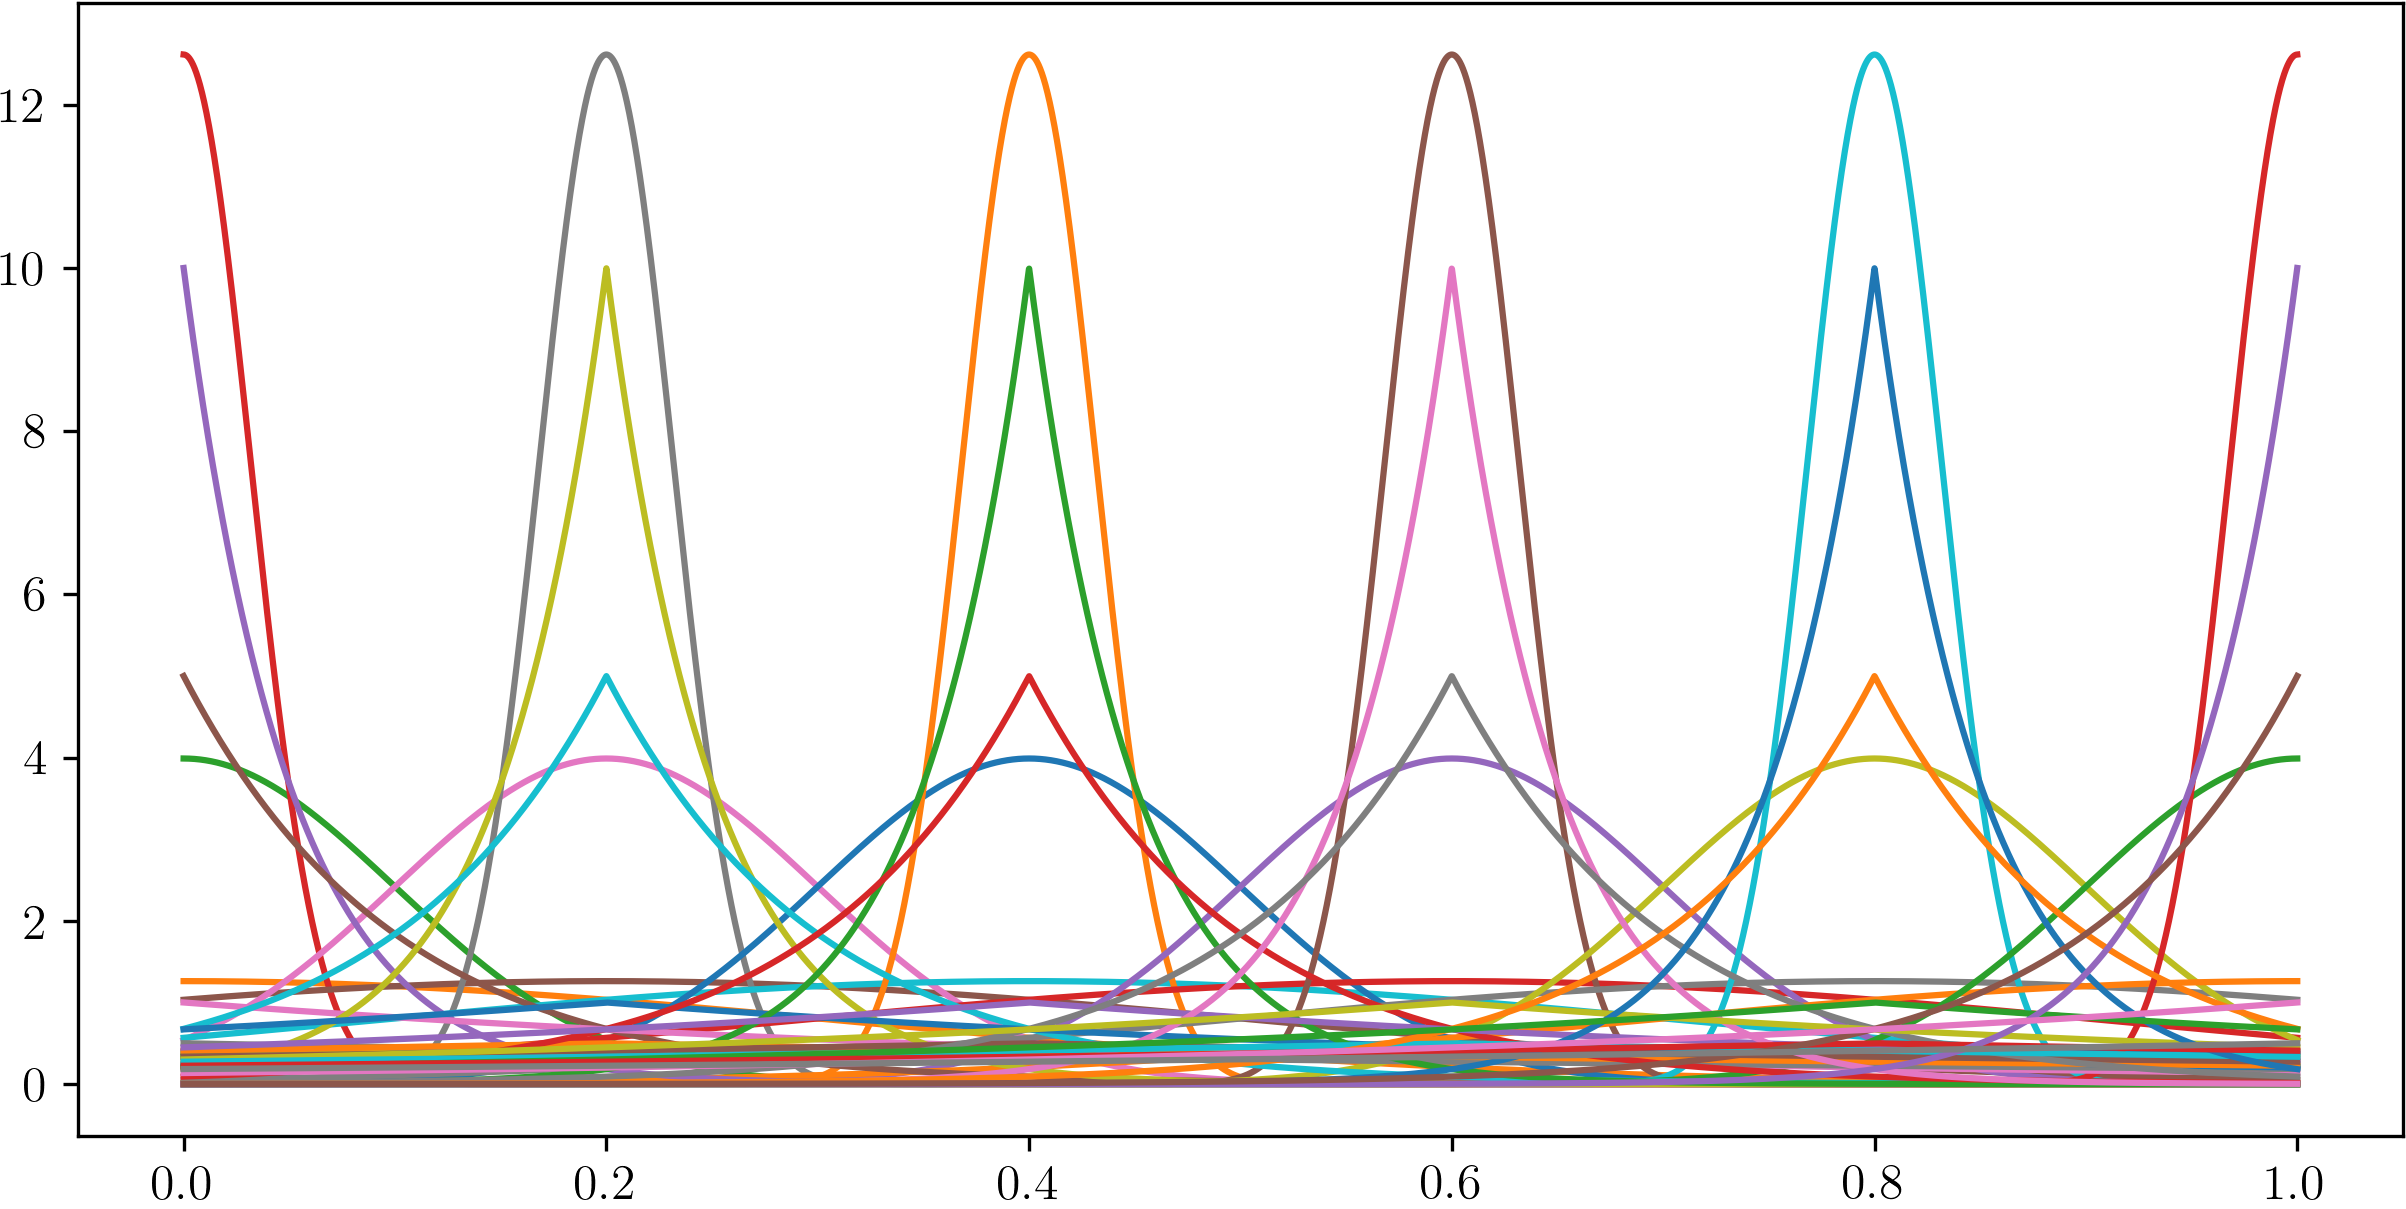
\includegraphics[width=1\textwidth]{TeX_files/lapl_gauss_dict.png}
\caption{$D_{GL}$, set of Gaussian and Laplace densities.}
\label{fig:dict}
\end{figure}
%\item Union of Fourier and Haar aud Gaussians ?
\item The second dictionary, denoted by $D_{GLU}$, is obtained by enriching
the first dictionary $D_{GL}$ by the set of $10$ uniform densities on the intervals 
$(i, i+0.1)$, $i\in \{0, 0.1,\dots,0.9\}$. This dictionary $D_{GLU}$ has 64 elements.
\end{enumerate}
A table of the dictionary $D_{GL}$ (and $D_{GLU}$ with the uniform densities) can be found in \Cref{table:densities_DGLU}.

\subsection{Densities considered}
We considered 5 target densities corresponding to 5 different scenarios. The $1^{st}$ and $2^{nd}$ will asses the performance of our method on uniform based densities, the $3^{rd}$ and $4^{th}$ on dictionary based density. The last one is a complex density made from elements which are not in the dictionary that we will consider.
\begin{enumerate}
\item{$f_{\textnormal{unif}}$:} A uniform density on $[0,1]$.
\item{$f_{\textnormal{rect}}$:} A mixture of uniform densities on subintervals. This density is called ``Rectangular'':
\begin{equation}
    f_{\textnormal{rect}}=\frac{10}{7}\b1_{[0,1/5]}+\frac{5}{7}\b1_{[1/5,2/5]}+
    \frac{10}{7}\b1_{[2/5,3/5]}+\frac{10}{7}\b1_{[4/5,1]}.
\end{equation}
\item{$f_{\textnormal{gauss}}$:} A mixture of 5 Gaussian densities taken from the dictionary $D_{GL}$ equally centered in $[0,1]$ with same variance:
\begin{equation}
    f_{\textnormal{gauss}}=\sum_{k=1}^5 0.2f_{k} \quad \text{with}\quad f_k=\varphi_{(k/5,0.001)}.
\end{equation}

\item{$f_{\textnormal{gauss-lapl}}$:} A mixture of 5 Gaussian and Laplace densities taken from the dictionary $D_{GL}$ with different variances and scales:
%(multivariate_normal(0.2, 10**(-3)))
%(multivariate_normal(0.6, 10**(-3)))
%(multivariate_normal(0, 10**(-2)))
%(laplace(0.4,0.2))
%(laplace(0.8,0.1))
\begin{equation}
\begin{array}{ll}
f_{\textnormal{gauss-lapl}}=0.2\big(&\varphi_{(0 ,10^{-2})} + \varphi_{(0.2,10^{-3})}+\varphi_{(0.6,10^{-3})}\\
    &+\text{\small Lapl}_{(0.4,0.2)}+\text{\small Lapl}_{(0.8,0.1)} \big).
\end{array}
\end{equation}
\item{$f_{\textnormal{ext}}$:} A mixture of Gaussian and Laplace densities taken from another dictionary $D_{out}$:
%append(multivariate_normal(0.1, 5*10**(-3)))
%append(multivariate_normal(0.65, 10**(-3)))
%append(multivariate_normal(0.9, 10**(-2)))
%append(laplace(0.5, 0.08))
%append(laplace(0.2, 0.07))
%append(laplace(0.75, 0.05))

\begin{equation}
    f_{\textnormal{ext}}=\sum_{k=1}^7 \frac{1}{7}f_{k} \quad \text{with}\quad f_k\in D_{out}.
\end{equation}
\end{enumerate}
These target densities are plotted in \Cref{fig:target_densities}.
\begin{figure}[h]
\center
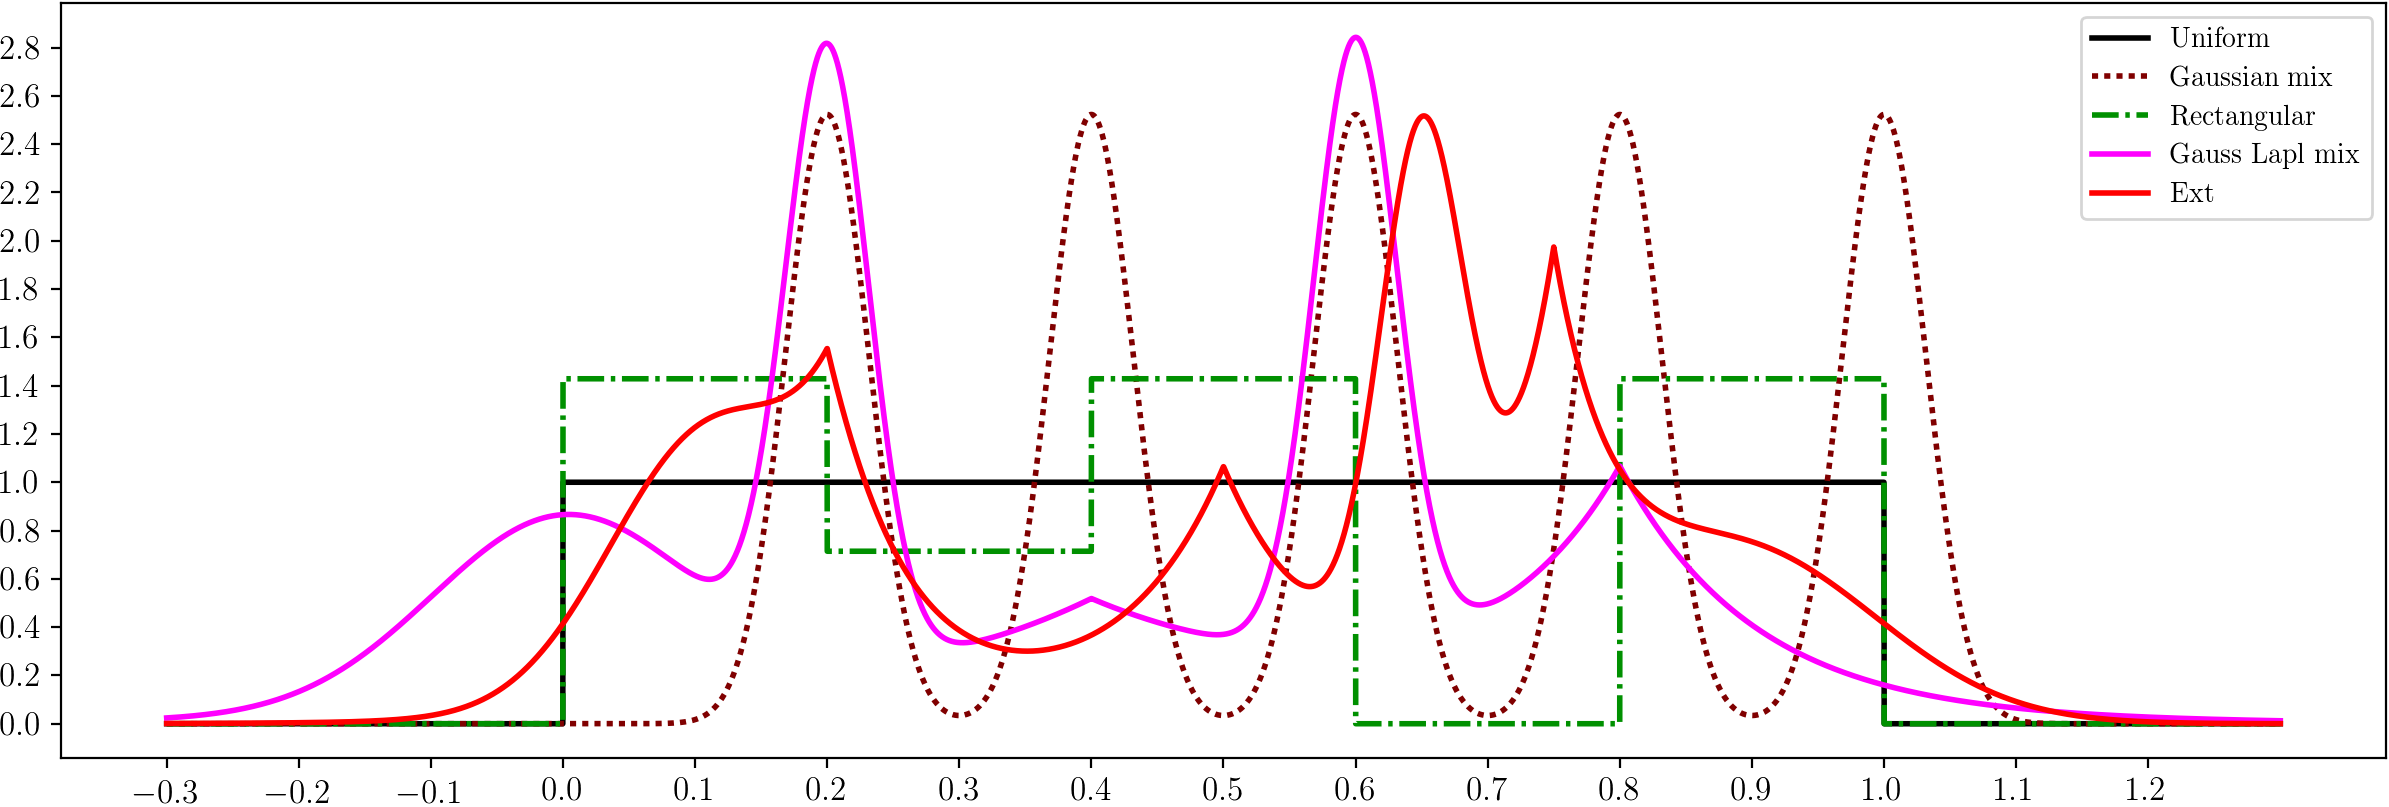
\includegraphics[width=\textwidth]{TeX_files/densities_f_star.png}
\caption{Five target densities considered in the experiments.}
\label{fig:target_densities}
\end{figure}

\subsection{Discussion of the results}

In the numerical experiments reported in this section, the dictionaries used for the Adaptive Dantzig 
and the Maximum likelihood density estimators are $D_{GL}$ and $D_{GLU}$. Note that the AD is the direct 
competitor of the MLE as both methods rely on a dictionary. However, in order to get a broader insight of
what is going on, we also compared these dictionary based methods with other commonly used density 
estimators such as the EM algorithm on Gaussian mixtures with a model selection performed by the BIC 
criterion and Kernel Density Estimators (KDE). In the plots, KDE refers to the kernel density estimate 
with Scott's rule as chosen by default in the Python library Scipy, KDE-SJ refers to the KDE with the 
Sheather-Jones bandwidth selector and KDE CV refers to the KDE with bandwidth selected via cross-validation. 
The two latter were implemented by ourselves. 

For each scenario of the target density, $f_{\textnormal{unif}}$, $f_{\textnormal{rect}}$, 
$f_{\textnormal{gauss}}$, $f_{\textnormal{gauss-lapl}}$, $f_{\textnormal{ext}}$ and for each sample size $N$  
with $N\in\{100, 500, 1000\}$, we ran 200 simulations. The boxplots of the errors are plotted in 
\Cref{fig:res_ext_L2_GL}-\Cref{fig:res_ext_KL_GLU}. The running times of different arguments are 
depicted in \Cref{fig:res_times}. A rapid observation is that the performance of the MLE is good both 
in Kullback-Leibler and $L_2$ losses, and it outperforms in all considered scenarios the 
AD estimator. This is true both in terms of statistical accuracy and computational complexity. 
The comparison with the other estimation methods is more subtle, and requires a closer look
to the results.

\subsubsection{Mis-specification bias}

Obviously, the densities $f_{\textnormal{unif}}$, $f_{\textnormal{rect}}$ and $f_{\textnormal{ext}}$ 
were not built with elements in the dictionary $D_{GL}$. In other terms, they do not lie in the convex hull
of the dictionary $D_{GL}$. Furthermore, they can be hardly approximated by convex combinations of functions
from $D_{GL}$. Therefore, it is clear that whatever the dictionary based approach we use, it will have a 
significant bias due to the ``model mis-specification''. 


%Uniform, rect, ext
\begin{figure}
\center
    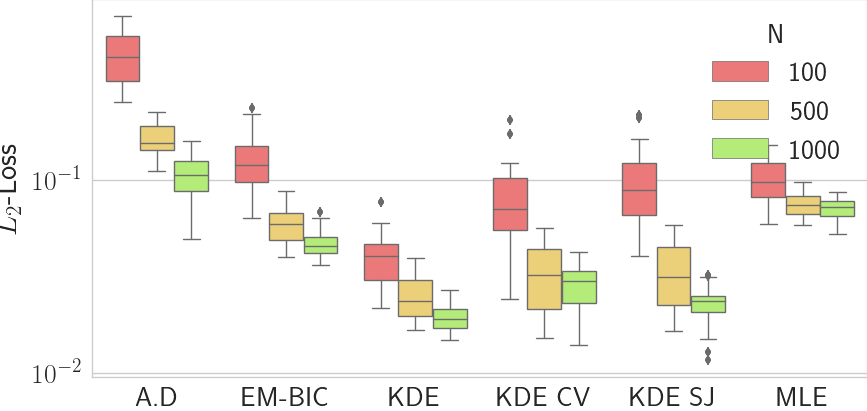
\includegraphics[width=0.8\textwidth]{./TeX_files/res_uniform_L2_GL.png}
    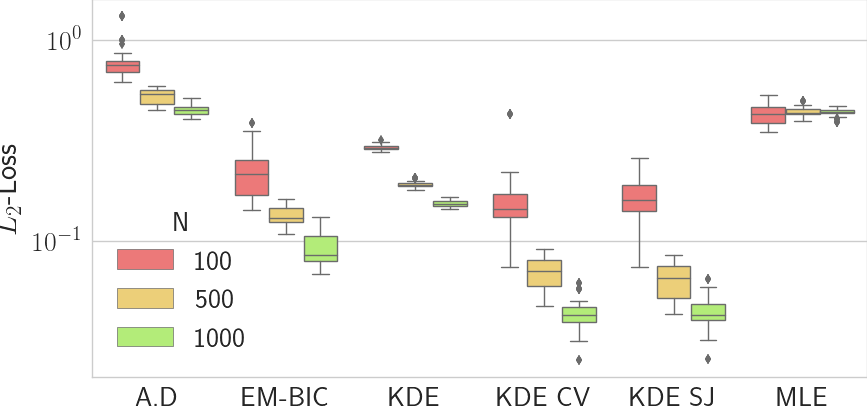
\includegraphics[width=0.8\textwidth]{./TeX_files/res_rect_L2_GL.png}
    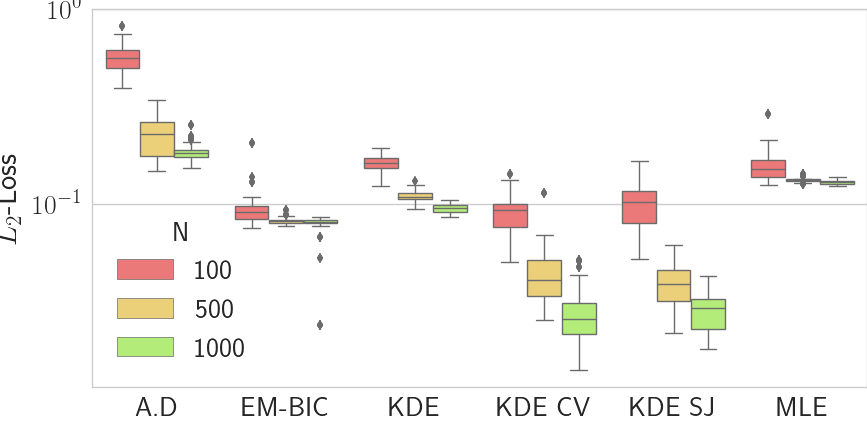
\includegraphics[width=0.8\textwidth]{./TeX_files/res_lapl_gauss_not_dict_L2_GL.png}
    \caption{Results with $f_{\textnormal{unif}}$ (upper panel), $f_{\textnormal{rect}}$ 
    (middle panel) and $f_{\textnormal{ext}}$ (lower panel) in $L2$ loss with $D_{GL}$.}
    \label{fig:res_ext_L2_GL}
\end{figure}

Since the cardinality of the dictionary is chosen
independently of the sample size $n$, this bias term is constant across different values of $n$. This is 
exactly what we observe in \Cref{fig:res_ext_L2_GL}. Such methods as the EM-BIC or various versions of KDE
have an $L_2$ error that decreases significantly when the sample size increases, whereas the AD and, especially, 
the MLE show only a slight improvement of the error. This is a strong indication of the fact that
the bias of the methods AD and MLE substantially dominates the bias, when the true density is chosen from 
the set $\{f_{\textnormal{unif}},\,f_{\textnormal{rect}},\,f_{\textnormal{ext}}\}$. Thus, the apparently
poor behavior of the MLE as compared to the EM-BIC and the KDE is not a surprise and, more importantly,
it is not caused by the method of estimation itself but rather by the inappropriate choice of the
dictionary.

Note that in all the experiments, the conclusions drawn from the error bars corresponding to the 
$L_2$-error can be drawn from the error bars corresponding to the KL-error. 

\begin{figure}
\center
    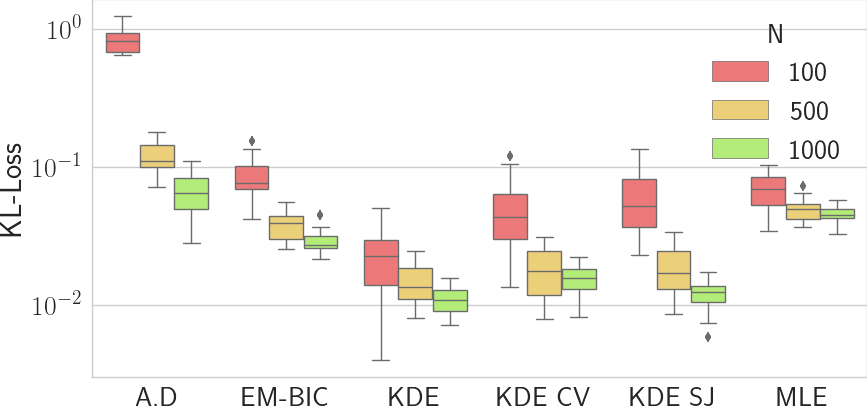
\includegraphics[width=0.8\textwidth]{./TeX_files/res_uniform_KL_GL.png}
    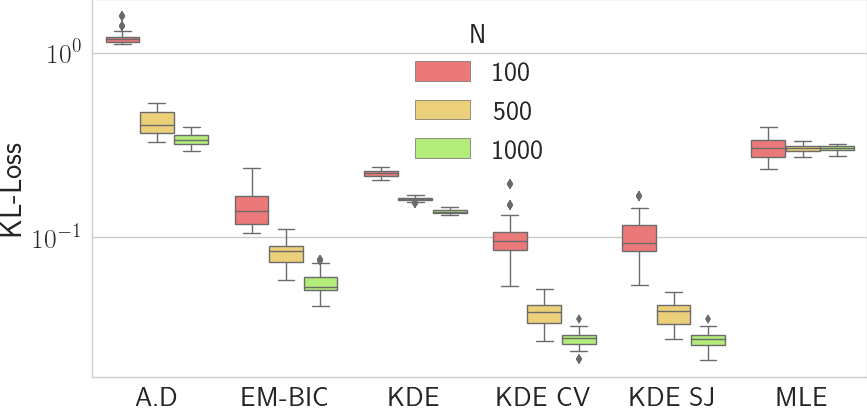
\includegraphics[width=0.8\textwidth]{./TeX_files/res_rect_KL_GL.png}
    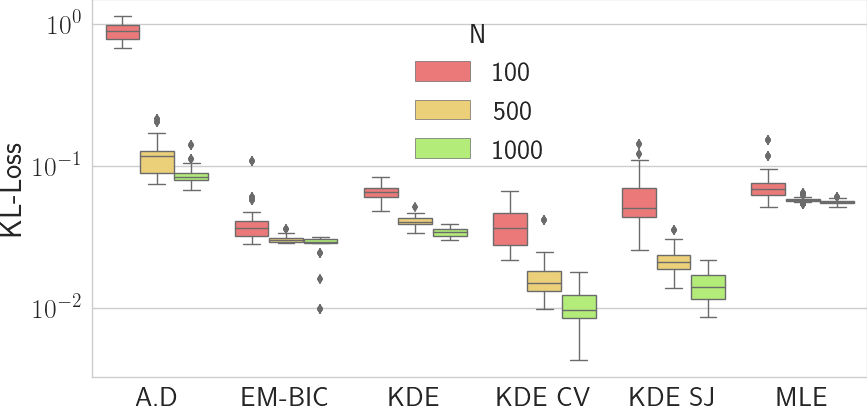
\includegraphics[width=0.8\textwidth]{./TeX_files/res_lapl_gauss_not_dict_KL_GL.png}
    \caption{Results with $f_{\textnormal{unif}}$ (upper panel), $f_{\textnormal{rect}}$ 
    (middle panel) and $f_{\textnormal{ext}}$ (lower panel) in KL loss with $D_{GL}$.}
    \label{fig:res_ext_KL_GL}
\end{figure}

\subsubsection{Assessing estimation error}

While for the three densities discussed in the foregoing paragraph the bias was largely dominating 
the variance, the situation is reversed for the densities $f_{\textnormal{gauss}}$ and 
$f_{\textnormal{gauss-lapl}}$. Both of them belong to the convex hull of the dictionary 
$D_{GL}$, which implies that the mis-specification bias vanishes. Therefore, the error
is mostly dominated by the estimation variance. This explains why for these two densities
the MLE has the smallest error, both in $L_2$ and KL loss (see \Cref{fig:res_lapl_gauss_L2_GL} 
and \Cref{fig:res_lapl_gauss_KL_GL}). Interestingly, the second best is EM-BIC, which performs 
better than the AD. Note that the default KDE in Scipy \citep{scipy} with Scott's rule 
presents poor results in these scenarios. This observation should come to mind of the 
practitioner when applying kernel density estimators with default package setting. 

One can also remark that the error of the MLE when estimating $f_{\textnormal{gauss}}$
is smaller than the one of estimating $f_{\textnormal{gauss-lapl}}$. This is perfectly
in line with the theory developed in previous chapter, telling that the variance term
is proportional to the sparsity index. In these examples, the sparsity index of 
$f_{\textnormal{gauss-lapl}}$ is larger than that of $f_{\textnormal{gauss}}$.

%gauss
\begin{figure}
\center
    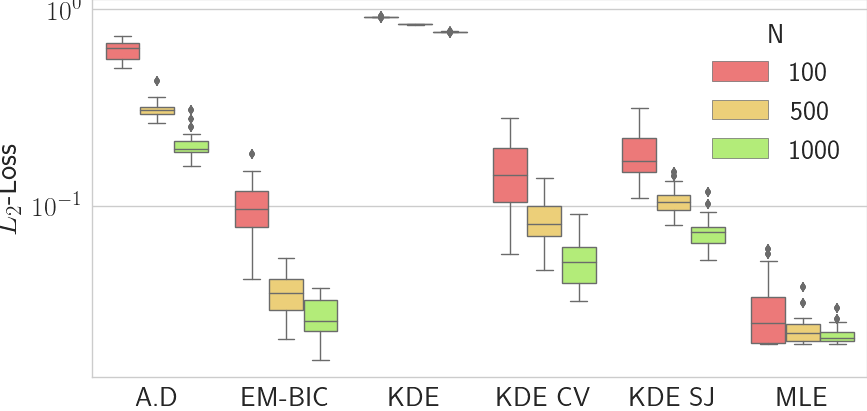
\includegraphics[width=0.8\textwidth]{./TeX_files/res_gauss_L2_GL.png}
    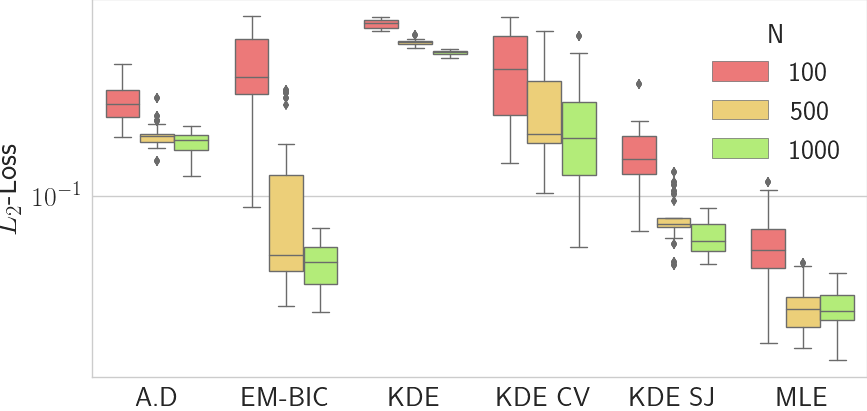
\includegraphics[width=0.8\textwidth]{./TeX_files/res_lapl_gauss_L2_GL.png}
    \caption{Results with $f_{\textnormal{gauss}}$ (upper panel) and $f_{\textnormal{gauss-lapl}}$ 
    (lower panel) in $L_2$ loss with $D_{GL}$.}
    \label{fig:res_lapl_gauss_L2_GL}
\end{figure}

\begin{figure}
\center
    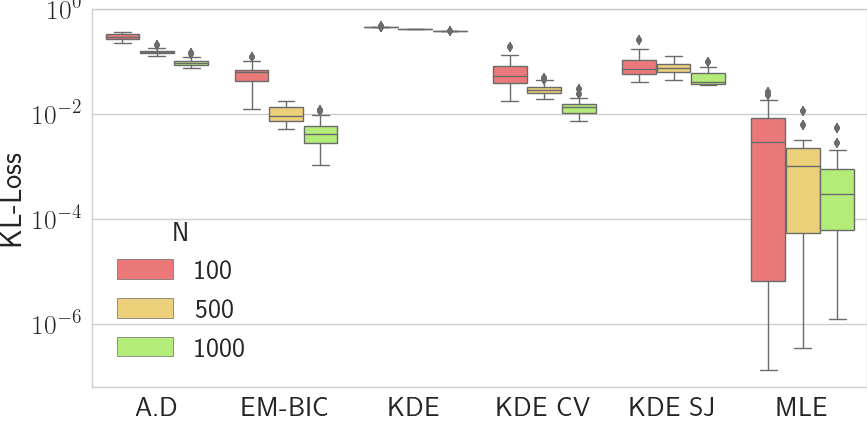
\includegraphics[width=0.8\textwidth]{./TeX_files/res_gauss_KL_GL.png}
    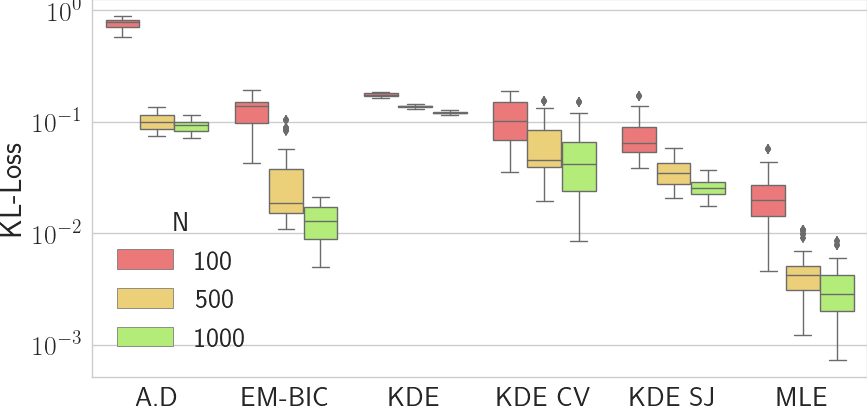
\includegraphics[width=0.8\textwidth]{./TeX_files/res_lapl_gauss_KL_GL.png}
    \caption{Results with $f_{\textnormal{gauss}}$ (upper panel) and $f_{\textnormal{gauss-lapl}}$ 
    (lower panel) in KL loss with $D_{GL}$.}
    \label{fig:res_lapl_gauss_KL_GL}
\end{figure}


\subsubsection{Impact of the choice of the dictionary \label{dict_dglu_sect}}

The discussion of the foregoing paragraphs demonstrates the importance of the choice of the dictionary.
The purpose of the additional experiments conducted with the same target densities but with a larger dictionary, $D_{GLU}$,
is to further illustrate this importance and to show that the size of the dictionary does not significantly impact 
the quality of estimation\footnote{It certainly does impact the running time}.

The inclusion of  $10$ uniform densities on $(0,0.1),\dots,(0.9,1)$ to the dictionary $D_{GL}$ removes the mis-specification
bias in the case of a uniform and rectangular densities, and reduces it in the case of $f_{\textnormal{ext}}$.
The results are plotted in \Cref{fig:res_gauss_L2_GLU} and \Cref{fig:res_gauss_KL_GLU}. 
We can see that the MLE becomes generally the best estimator when the density is uniform or rectangular. 
It is still slightly worse than the KDE with data-driven bandwidths for estimating $f_{\textnormal{ext}}$.
 \begin{figure}
\center
    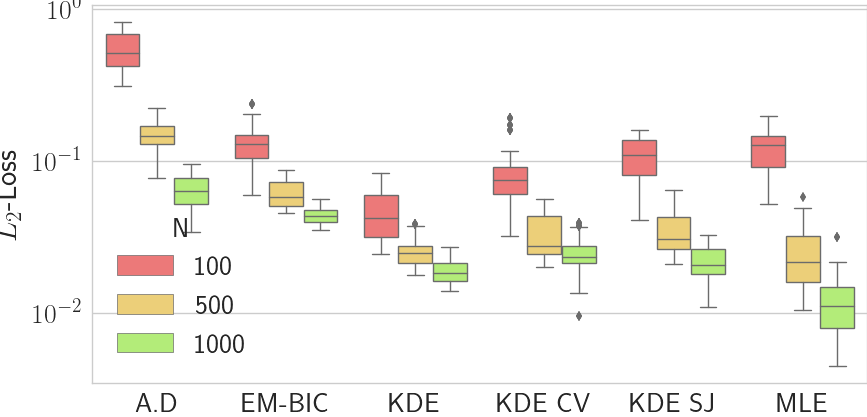
\includegraphics[width=0.8\textwidth]{./TeX_files/res_uniform_L2_GLU.png}
    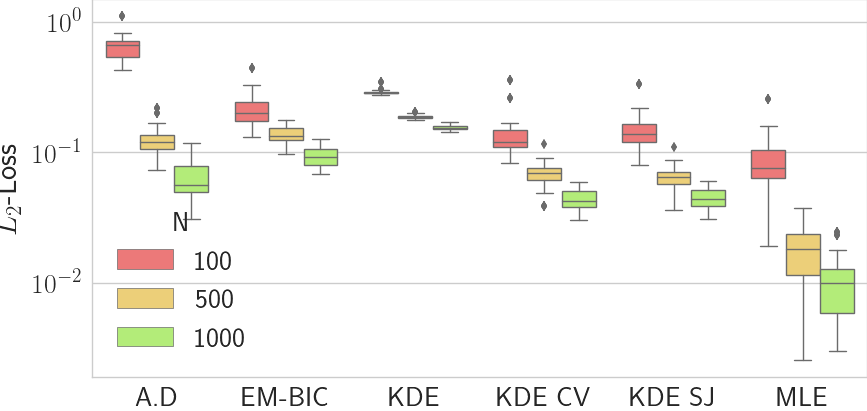
\includegraphics[width=0.8\textwidth]{./TeX_files/res_rect_L2_GLU.png}
    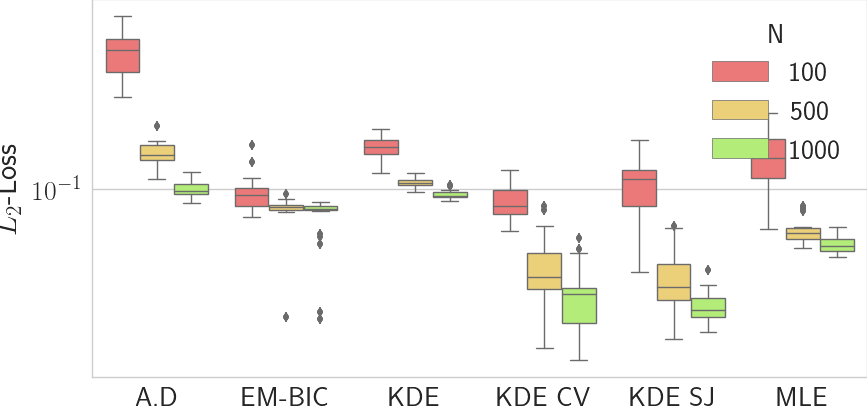
\includegraphics[width=0.8\textwidth]{./TeX_files/res_lapl_gauss_not_dict_L2_GLU.png}
    \caption{Results with $f_{\textnormal{unif}}$ (upper panel), $f_{\textnormal{rect}}$ 
    (middle panel) and $f_{\textnormal{ext}}$ (lower panel) in $L_2$ loss with $D_{GLU}$.}
    \label{fig:res_gauss_L2_GLU}
\end{figure}
Finally, the results for the densities $f_{\textnormal{gauss}}$ and $f_{\textnormal{gauss-lapl}}$
plotted on \Cref{fig:res_ext_L2_GLU} and \Cref{fig:res_ext_KL_GLU} confirm that
adding new elements to the dictionary (even if they are ``useless'') do not deteriorate
the quality of estimation. The $\ell_1$-constraint allow us to avoid the overfitting. 
\begin{figure}
\center
    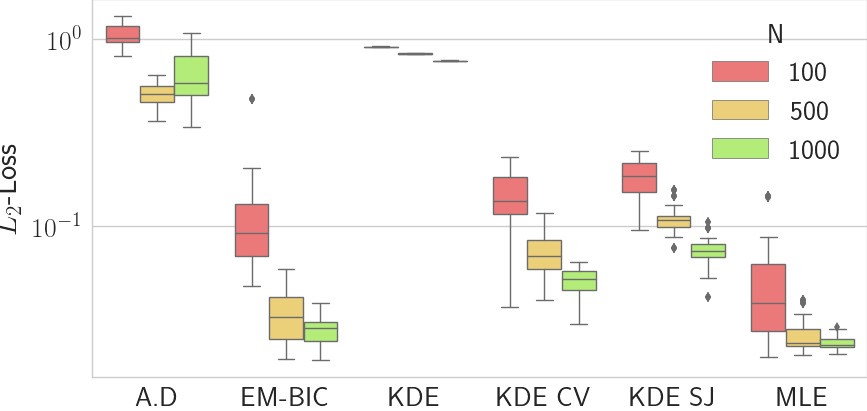
\includegraphics[width=0.8\textwidth]{./TeX_files/res_gauss_L2_GLU.png}
    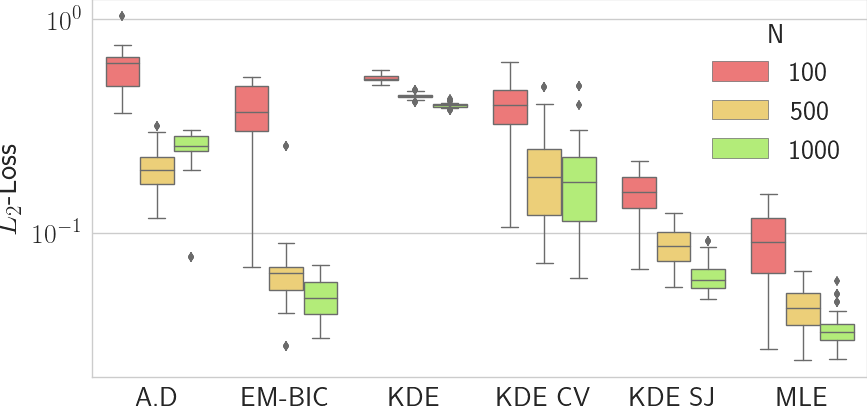
\includegraphics[width=0.8\textwidth]{./TeX_files/res_lapl_gauss_L2_GLU.png}
    \caption{Results with $f_{\textnormal{gauss}}$ (upper panel) and $f_{\textnormal{gauss-lapl}}$ 
    (lower panel) in $L2$ loss with $D_{GLU}$.}
    \label{fig:res_ext_L2_GLU}
\end{figure}

\subsubsection{Comparison of weights estimated by AD and MLE}

A closer look on the estimated weights by AD and MLE gives us knowledge on the behavior of these estimators. We considered the full dictionary $D_{GLU}$ and we provided a table of the indexes of components of this dictionary in \Cref{table:densities_DGLU}. We plotted the estimated weights of the true components of $f_{\textnormal{gauss}}$ and $f_{\textnormal{gauss-lapl}}$ in \Cref{fig:weights_gauss_real_indexes} and \Cref{fig:weights_gauss_laplace_real_indexes}. The MLE estimates correctly the real weights of $f_{\textnormal{gauss}}$ and most of the weights of $f_{\textnormal{gauss-lapl}}$. We recall the reader that those weights were set to $0.2$. However, AD did not succeed to estimate correctly these weights. It turns out that AD gave importance on components that overlap the true densities of the mixture as shown in \Cref{fig:weights_gauss_and_laplace_unif_indexes} with the uniform components. Both AD and MLE provide sparse estimators, this can be seen by looking at components not used in the dictionary (see \Cref{fig:weights_gauss_and_laplace_other_indexes}). As a matter of fact, the estimated weight vector by AD is more sparse that MLE, but AD is more prone to be influenced by overlapping densities.

\begin{figure}
\center
    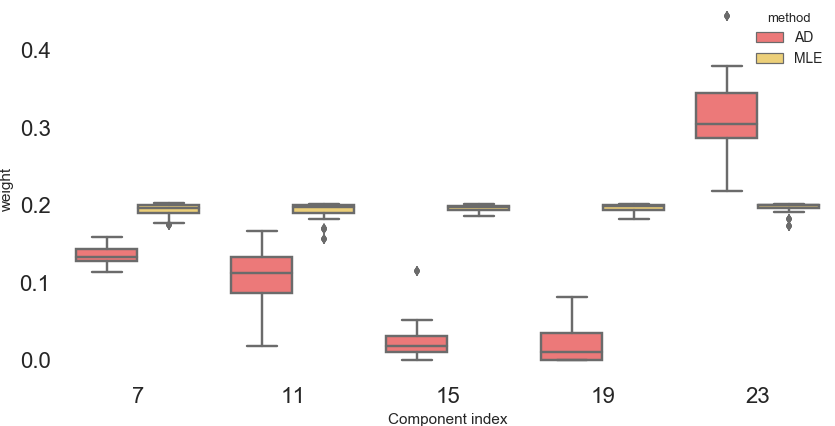
\includegraphics[width=0.8\textwidth]{./TeX_files/weight_f_gauss_real_comp_N_500.png}
    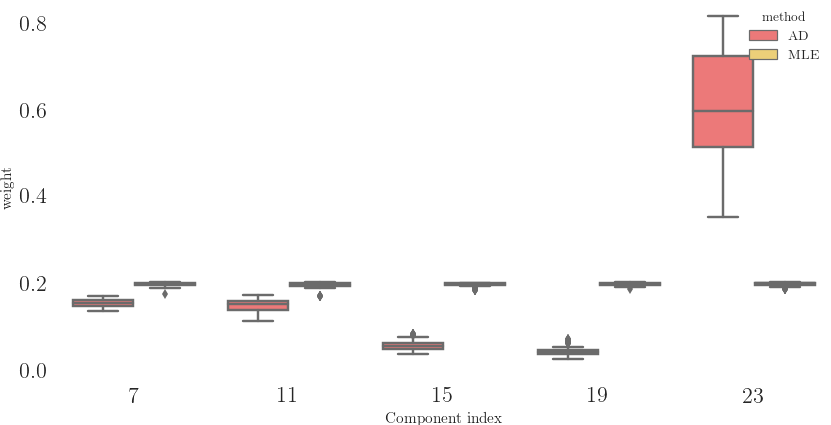
\includegraphics[width=0.8\textwidth]{./TeX_files/weight_f_gauss_real_comp_N_1000.png}
    \caption{Estimated weights of the components of $f_{\textnormal{gauss}}$, with $N=500$ (upper panel) and $N=1000$
    (lower panel).}
    \label{fig:weights_gauss_real_indexes}
\end{figure}
\begin{figure}
\center
    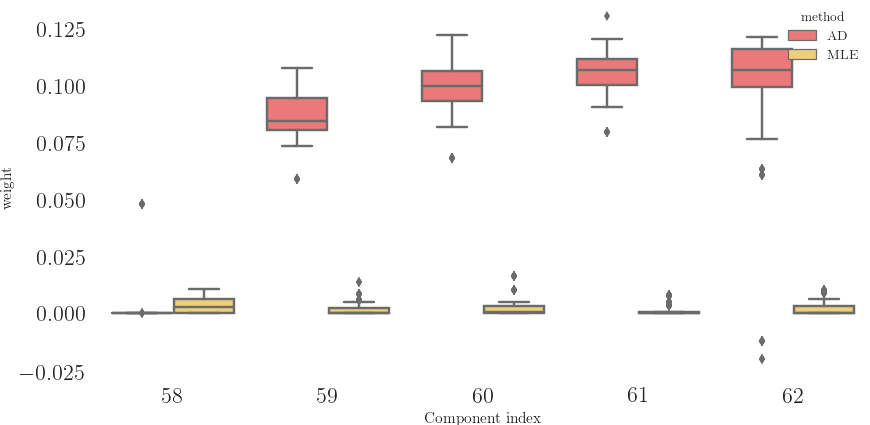
\includegraphics[width=0.8\textwidth]{./TeX_files/weight_f_gauss_unif_comp_N_1000.png}
    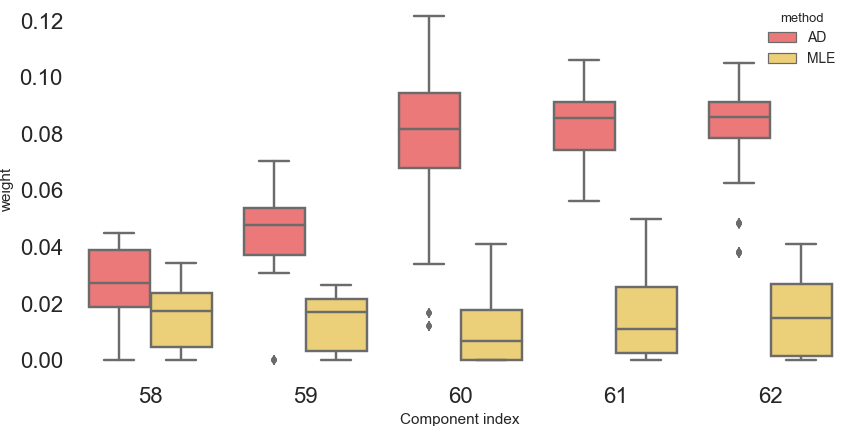
\includegraphics[width=0.8\textwidth]{./TeX_files/weight_f_gauss_laplace_unif_comp_N_1000.png}
    \caption{Estimated weights of uniform components of the dictionary for 
    $f_{\textnormal{gauss}}$ (upper panel) and $f_{\textnormal{gauss-lapl}}$ (lower panel) with $N=1000$.}
    \label{fig:weights_gauss_and_laplace_unif_indexes}
\end{figure}

\begin{figure}
\center
    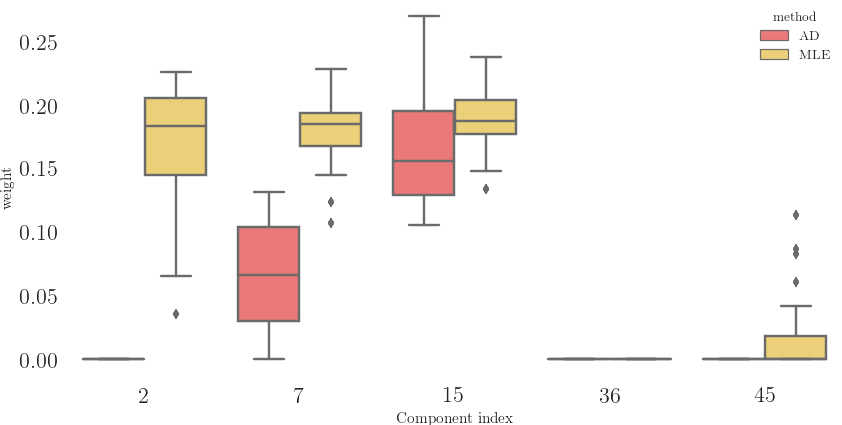
\includegraphics[width=0.8\textwidth]{./TeX_files/weight_f_gauss_laplace_real_comp_N_500.png}
    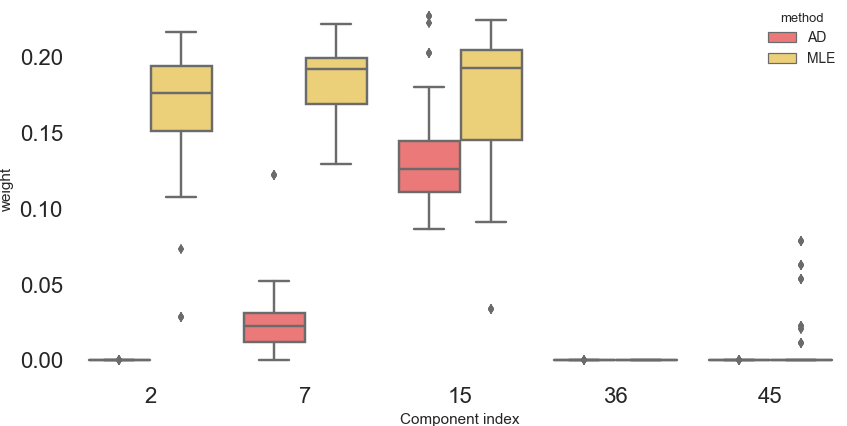
\includegraphics[width=0.8\textwidth]{./TeX_files/weight_f_gauss_laplace_real_comp_N_1000.png}
    \caption{Estimated weights of the components of $f_{\textnormal{gauss-lapl}}$, with $N=500$ (upper panel) and $N=1000$
    (lower panel).}
    \label{fig:weights_gauss_laplace_real_indexes}
\end{figure}
\begin{figure}
\center
    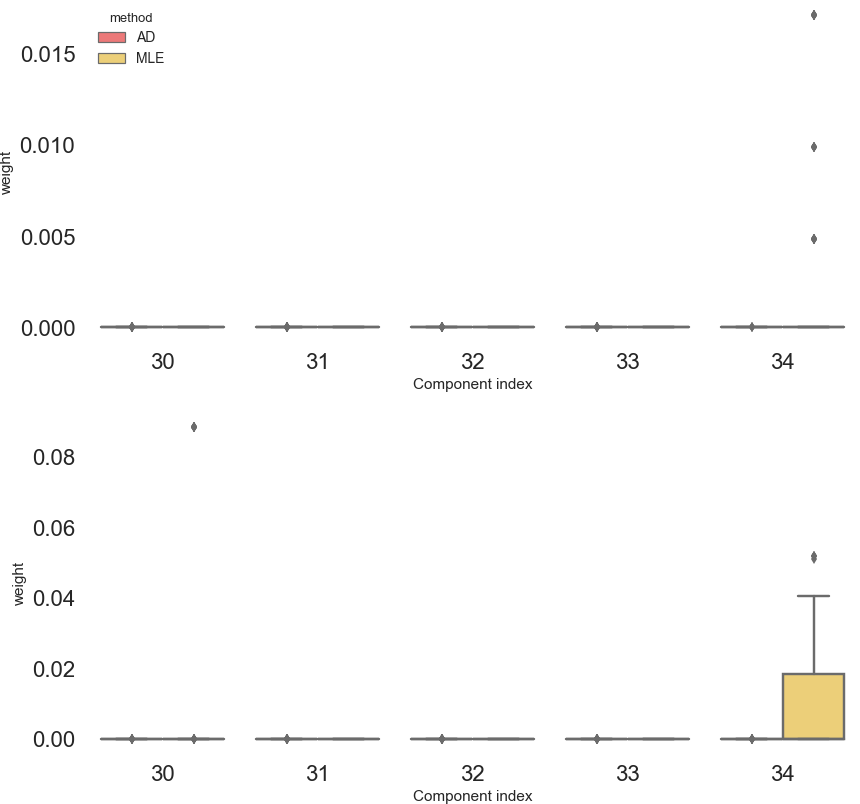
\includegraphics[width=0.8\textwidth]{./TeX_files/weight_f_gauss_and_laplace_other_comp_N_1000.png}
    \caption{Estimated weights of non-used components of the dictionary for  $f_{\textnormal{gauss}}$ (upper panel) and $f_{\textnormal{gauss-lapl}}$ (lower panel), with $N=1000$.}
    \label{fig:weights_gauss_and_laplace_other_indexes}
\end{figure}

\begin{figure}
\center
\begin{tabular}{|c|l|c|l|c|l|}
\hline
0 & Normal( 0 , 1 ) &22 & Normal( 1 , 0.01 ) &44 & Laplace( 0.8 , 0.05 ) \\ \hline
1 & Normal( 0 , 0.1 ) &23 & Normal( 1 , 0.001 ) &45 & Laplace( 0.8 , 0.1 ) \\ \hline
2 & Normal( 0 , 0.01 ) &24 & Laplace( 0 , 0.05 ) &46 & Laplace( 0.8 , 0.2 ) \\ \hline
3 & Normal( 0 , 0.001 ) &25 & Laplace( 0 , 0.1 ) &47 & Laplace( 0.8 , 0.5 ) \\ \hline
4 & Normal( 0.2 , 1 ) &26 & Laplace( 0 , 0.2 ) &48 & Laplace( 0.8 , 1 ) \\ \hline
5 & Normal( 0.2 , 0.1 ) &27 & Laplace( 0 , 0.5 ) &49 & Laplace( 1 , 0.05 ) \\ \hline
6 & Normal( 0.2 , 0.01 ) &28 & Laplace( 0 , 1 ) &50 & Laplace( 1 , 0.1 ) \\ \hline
7 & Normal( 0.2 , 0.001 ) &29 & Laplace( 0.2 , 0.05 ) &51 & Laplace( 1 , 0.2 ) \\ \hline
8 & Normal( 0.4 , 1 ) &30 & Laplace( 0.2 , 0.1 ) &52 & Laplace( 1 , 0.5 ) \\ \hline
9 & Normal( 0.4 , 0.1 ) &31 & Laplace( 0.2 , 0.2 ) &53 & Laplace( 1 , 1 ) \\ \hline
10 & Normal( 0.4 , 0.01 ) &32 & Laplace( 0.2 , 0.5 )&54 & Uniform( 0.0 , 0.1 ) \\ \hline
11 & Normal( 0.4 , 0.001 ) &33 & Laplace( 0.2 , 1 )&55 & Uniform( 0.1 , 0.2 ) \\ \hline
12 & Normal( 0.6 , 1 ) &34 & Laplace( 0.4 , 0.05 )&56 & Uniform( 0.2 , 0.3 ) \\ \hline
13 & Normal( 0.6 , 0.1 ) &35 & Laplace( 0.4 , 0.1 )&57 & Uniform( 0.3 , 0.4 ) \\ \hline
14 & Normal( 0.6 , 0.01 ) &36 & Laplace( 0.4 , 0.2 )&58 & Uniform( 0.4 , 0.5 ) \\ \hline
15 & Normal( 0.6 , 0.001 ) &37 & Laplace( 0.4 , 0.5 )&59 & Uniform( 0.5 , 0.6 ) \\ \hline
16 & Normal( 0.8 , 1 ) &38 & Laplace( 0.4 , 1 )&60 & Uniform( 0.6 , 0.7 ) \\ \hline
17 & Normal( 0.8 , 0.1 ) &39 & Laplace( 0.6 , 0.05 )&61 & Uniform( 0.7 , 0.8 ) \\ \hline
18 & Normal( 0.8 , 0.01 ) &40 & Laplace( 0.6 , 0.1 )&62 & Uniform( 0.8 , 0.9 ) \\ \hline
19 & Normal( 0.8 , 0.001 ) &41 & Laplace( 0.6 , 0.2 )&63 & Uniform( 0.9 , 1.0 ) \\ \hline
20 & Normal( 1 , 1 ) &42 & Laplace( 0.6 , 0.5 )& &   \\ \hline
21 & Normal( 1 , 0.1 ) &43 & Laplace( 0.6 , 1 )& &   \\ \hline
\end{tabular}
\caption{Indexes of components of the dictionary $D_{GL}$ and $D_{GLU}$ }
\label{table:densities_DGLU}
\end{figure}

\subsubsection{Concluding remarks} 

To conclude, the performance of the MLE method in these simulations is promising to achieve a 
good mixture density estimate. In addition, the computational efficiency of the MLE displayed in 
\Cref{fig:res_times} makes it highly attractive for performing density estimation. Our algorithm 
was coded in Python with some elements accelerated with the Just-In-Time (JIT) compiler Numba \citep{numba}. 
Compared to compiled optimized versions of KDE and EM from Scipy and Scikit-Learn\citep{scikit-learn}, 
we are confident that the computation time of our algorithm can be further decreased. Another important 
point is in the case of high dimensional data, KDE and EM+BIC methods are known to present poor 
performance. Our method needs the computation of the matrix $(f_j(X_i))_{(i,j)\in [N]\times [K]}$ 
which might consume a lot of memory. Some techniques such as a Mini-batch approach can help. 
Furthermore, at the light of the results in the uniform and rectangular case, the choice of the 
dictionary is a cornerstone in density estimation. The size of the dictionary should be chosen 
by considering both statistical arguments and computational limitations.


\begin{figure}
\center
    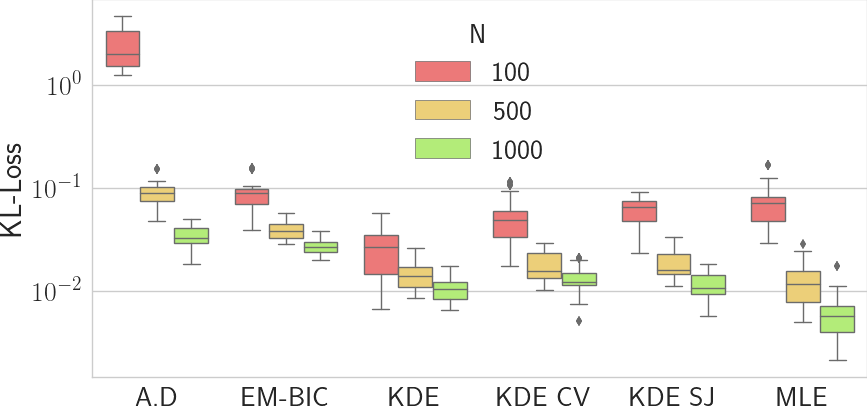
\includegraphics[width=0.8\textwidth]{./TeX_files/res_uniform_KL_GLU.png}
    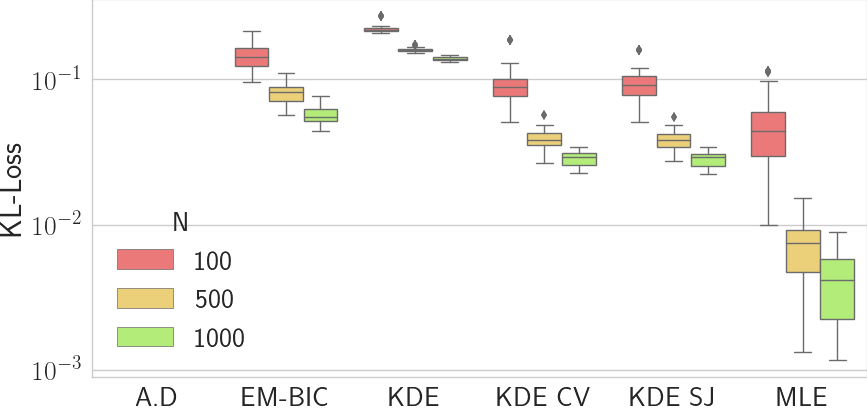
\includegraphics[width=0.8\textwidth]{./TeX_files/res_rect_KL_GLU.png}
    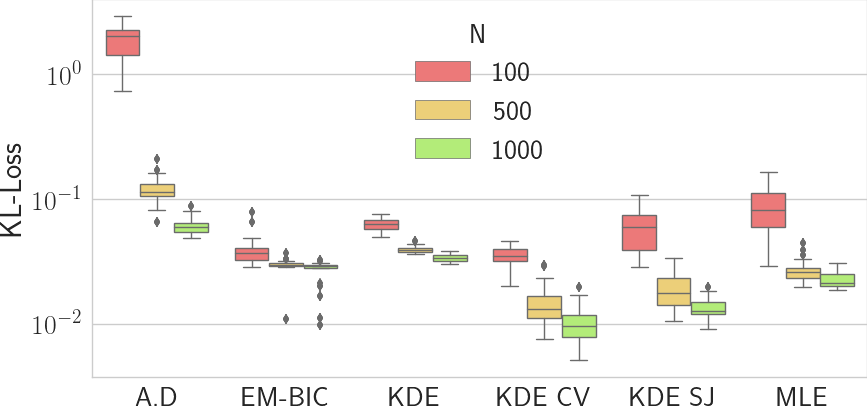
\includegraphics[width=0.8\textwidth]{./TeX_files/res_lapl_gauss_not_dict_KL_GLU.png}
    \caption{Results with $f_{\textnormal{unif}}$ (upper panel), $f_{\textnormal{rect}}$ 
    (middle panel) and $f_{\textnormal{ext}}$ (lower panel) in KL loss with $D_{GLU}$.}
    \label{fig:res_gauss_KL_GLU}
\end{figure}   
%lapl_gauss
\begin{figure}
\center
    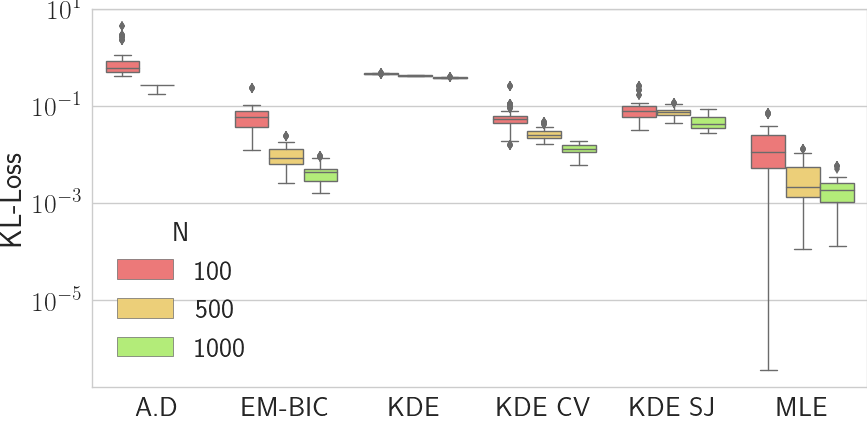
\includegraphics[width=0.8\textwidth]{./TeX_files/res_gauss_KL_GLU.png}
    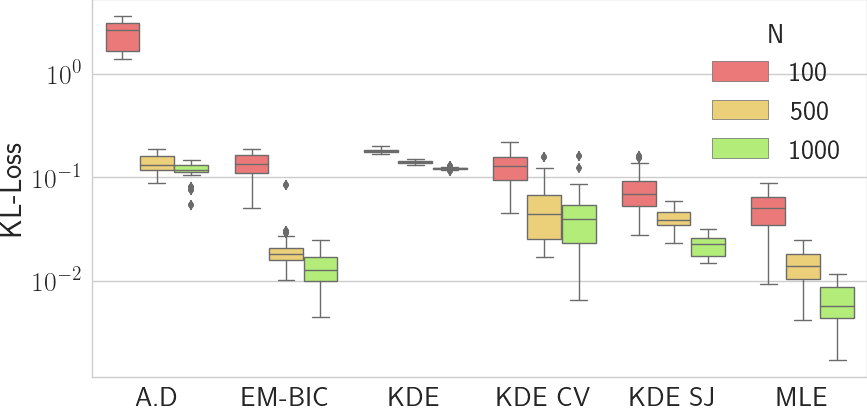
\includegraphics[width=0.8\textwidth]{./TeX_files/res_lapl_gauss_KL_GLU.png}
    \caption{Results with $f_{\textnormal{gauss}}$ (upper panel) and $f_{\textnormal{gauss-lapl}}$ 
    (lower panel) in KL loss with $D_{GLU}$.}
    \label{fig:res_ext_KL_GLU}
\end{figure} 


\begin{figure}
\center
    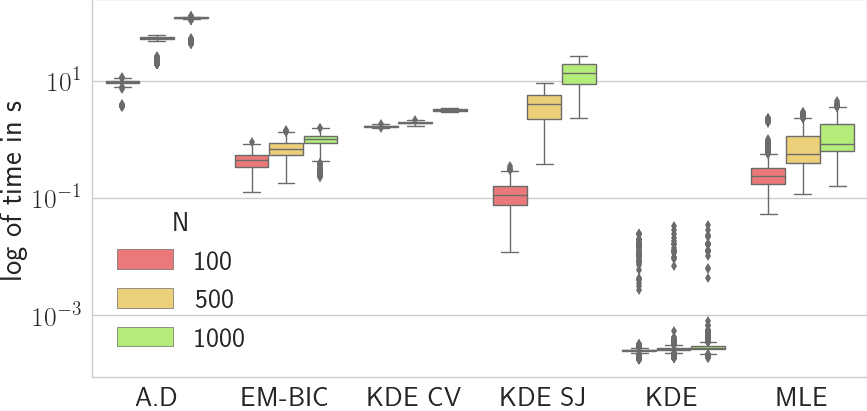
\includegraphics[width=0.8\textwidth]{./TeX_files/res_times.png}
    \caption{Computation times}
    \label{fig:res_times}
\end{figure}

\section{A method for constructing the dictionary of densities}
\label{sec:method_dict_gen}

In this section, we propose a data-driven method to construct a dictionary of densities for the KL-aggregation algorithm. We compare mixture densities estimated by this dictionary generation method and the KL-aggregation algorithm with the Kernel density estimator with the bandwidth selected via cross-validation and the Expectation-Maximization algorithm with the BIC criterion in different dimensional settings. We show experimentally that the KL-aggregation algorithm with a dictionary provided by this method offers good performance at an attractive computation cost.

\subsection{Implementation of the dictionary generator}

Given a sample $\bX_1,\dots,\bX_n\in\RR^p$, we construct the set of principal components $C$ of the design matrix $\bX$ by PCA. Then we build the set $S$ of all subspaces spanned by two elements of $C$:
\begin{equation}
  S = \{\textnormal{span}(\bv_i,\bv_j),\, (\bv_i,\bv_j) \in C.\}.
\end{equation}
On each subspace of $S$, we perform a clustering to find groups. For each group, we consider the points assigned to it in the original space and recover the empirical mean, the sample variance and construct a normal density with these parameters. A simple implementation would consider all principal components and thus $\frac{p(p-1)}{2}$ subspaces. On each of these subspace a clustering method such as K-means with an arbitrary large number of clusters K would be applied. The whole complexity would be $\mathcal{O}(p^2n^{2K+1})$. To reduce the computational complexity of this procedure, especially in high dimension, we adopted three strategies:
\begin{enumerate}
  \item Select the most informative components obtained via the PCA. One can use different techniques such as the Truncated SVD or the method proposed in \citep{Gavish2014} which circumvent the issue of not knowing $\textnormal{rank}(\bX)$. They considered the recovery of low-rank matrices from noisy data by hard thresholding of singular values by studying the asymptotic MSE. The AMSE-optimal choice of hard threshold would be for a $n$-by-$p$ matrix with $n\neq p$, $\hat\tau_* = \omega(\beta).y_{med}$, with $\beta = n/p$, $y_{med}$ is the median singular value of $\bX$ and $\omega(\beta)$ is described in \citep{Gavish2014}. An approximation of $\omega(\beta)$ is $\omega(\beta) \approx 0.56\beta^3 - 0.95\beta^2 + 1.82\beta + 1.43$. 
  \item Perform a model selection for each clustering which reduces the number of densities added to the dictionary. The method chosen is EM with BIC. 
  \item We address the problem of density duplicates in the dictionary originating from the same subset of points. We saw in the previous section that overlapping densities can degrade the performance of our estimators. One would like to remove these similar densities by performing a two-sample test. The reduction of multivariate two-sample testing to a binary classification problem follows from Friedman in \citep{Friedman:2003id}. To test whether two densities $P$ and $Q$ are equal, we draw two samples $\{\by_1,\dots,\by_n\}$ and $\{\bz_1,\dots,\bz_m\}$ from $P$ and $Q$ respectively and construct the dataset
\begin{equation}
  \mathcal{D} = \{(\bu_i,l_i)\}_{i=1}^{n+m}  \coloneqq  \{(\by_i,-1)\}_{i=1}^n \cup \{(\bz_i,0)\}_{i=1}^m.
\end{equation}
We shuffle $\mathcal{D}$ and keep a record of the original assignments for each sample in $\mathcal{D}$. Then, we split this dataset into two parts, $\mathcal{D}_{tr}$ for training a binary classifier and $\mathcal{D}_{te}$ for predicting the classification scores $\{s_i\}_{i=1}^{n+m}$. We consider the two sets $S_+$ and $S_-$, the first one contains the scores of the samples originating from $\{\bz_i\}_{i=1}^m$ and $S_-$ contains the scores of the samples originating from $\{\by_i\}_{i=1}^n$. We can view $S_+$ and $S_-$ as two samples drawn from two probability distributions, $p_+(s)$ and $p_-(s)$, and  apply a goodness-of-fit test such as the univariate Kolmogorov–Smirnov test, for testing the equality of these two densities. The resulting test statistic is the statistic for the multivariate two-sample test for the equality of the distributions $P$ and $Q$. 
\end{enumerate}
The dictionary construction procedure is given in \Cref{algo:dictionary_generator}

\begin{figure}[ht]
\begin{center}
\mybox{
\begin{minipage}{\linewidth}
\begin{algorithmic}%\SetAlgoLined\tt\SetLine
\small
\STATE {{\bfseries Input:} $\bX_1,\dots,\bX_n\textnormal{ with } \bX_i\in\RR^p$. And $K_{max}$, maximum number of clusters for EM-BIC, significance level $\alpha$.} 
\STATE {\bfseries Output:} A dictionary of densities $D=\{f_1,\dots,f_M\}$.
\STATE {\tt 1: Construct the set $\Omega$ of singular values of the design matrix $\bX\in\RR^{p\times n}$ which are greater than $\omega(\beta).y_{med}$ with $y_{med}$ median of singular values, $\beta = p/n$ and $\omega(\beta) \approx 0.56\beta^3 - 0.95\beta^2 + 1.82\beta + 1.43$.}
\STATE {\tt 2: Construct the set of principal components $\bar C$ corresponding to the singular values in $\Omega$.}
\FOR{ $\bv_i,\bv_j\in \bar C$ }
\STATE {\tt 3: Run EM-BIC with maximum $K_{max}$ clusters on the data projected to $\textnormal{span}(\bv_i, \bv_j)$, $\bX_1^{(i,j)},\dots,\bX_n^{(i,j)}$, and construct clusters of points $G_1,\dots,G_K$}.
\STATE {\tt 4: For each cluster $G_m$, $m\in [K]$, compute the mean $\hat\bmu_m$ and variance $\hat\bSigma_m$ of the points assigned to $G_m$ in the original space $\RR^P$}.
\STATE {\tt 5: Add to the dictionary $D$ the Gaussian densities $\{\varphi_{(\hat\bmu_m, \hat\bsigma_m)}\}_{m\in [K]}$.}
\ENDFOR.
\FOR{$\hat f_i, \hat f_j \in D$}
\STATE{\tt 6: Draw two samples $\{\by_1,\dots,\by_l\}, \{\bz_1,\dots,\bz_m\}$ from $\bY\sim \hat f_i$ and $\bZ\sim \hat f_j$ and construct the dataset $\mathcal{D} = \{(\bu_i,l_i)\}_{i=1}^{n+m}  \coloneqq  \{(\by_i,-1)\}_{i=1}^n \cup \{(\bz_i,0)\}_{i=1}^m.$}
\STATE{\tt 7: Shuffle and split $\mathcal{D}$ into $\mathcal{D}_{tr}$ and $\mathcal{D}_{te}$.}
\STATE{\tt 8: Train a binary classifier on $\mathcal{D}_{tr}$ and get the classification scores $\{s_i\}$ on $\mathcal{D}_{te}$.}
\STATE{\tt 9: Separate $\{s_i\}$ into $\{s_i\}^+$, scores of points drawn from $\bZ$ and $\{s_i\}^-$ for $\bY$.}
\STATE{\tt 10: Perform a two-samples Kolmogorov-Smirnov test on $\{s_i\}^+$ and $\{s_i\}^-$ and reject $H_0$ (The two multivariate samples are drawn from the same distribution) with significance level $\alpha$.}
\STATE{\tt 11: {\bf If} $H_0$ rejected, remove $\hat f_j$ of $D$, {\bf else}, keep $\hat f_i$ and $\hat f_j$.}
\ENDFOR.
\end{algorithmic}
\end{minipage}}
   \caption{Procedure for generating a dictionary of densities}
   \label{algo:dictionary_generator}
\end{center}
\end{figure}

\subsection{Experimental evaluation}

We created a mixture of 6 components in dimension 5, see \Cref{fig:experiments_data}, which mimics data that can be seen in real use cases. The simulation were run in dimension 3, 4 and 5 by selecting the corresponding first axis. We generated $N\in\{200, 500, 1000, 5000\}$ points and ran 200 simulations for each scenario (N, dimension). We used the dictionary generation procedure for the KL-aggregation algorithm with $K_{max} = 10$ on each subspaces and significance level $\alpha=0.05$. The dataset has been split into two equal parts, one for the dictionary generation algorithm and the other for the KL-aggregation algorithm. We compared the $L_2$-loss and KL-loss of our method to EM-BIC ($K_{max} = 20$) and KDE-CV (The bandwidth $h$ is selected via cross-validation in $[0.01, \dots, 1]$ in an equal partition of 20 elements). The computation times were also recorded. 

\subsubsection{ Results without the selection of principal components and the goodness-of-fit test for the dictionary generator algorithm.}

We compared, first, the KL-algorithm with the dictionary generated by our procedure to KDE-CV and EM-BIC without the two computation optimization techniques discussed before (selection of principal components and the deletion of similar densities). The time given for MLE is the total computational time of the generation of the dictionary and the aggregation algorithm. In the three scenarios (dimension 3,4 and 5), our algorithm presents same performance as EM-BIC in $L_2$ and KL loss with a better result when $N=5000$ (see \Cref{fig:result_dict_gen_dim_3,fig:result_dict_gen_dim_4,fig:result_dict_gen_dim_5}). Both methods outperforms KDE-CV in all scenarios. This indicates that the set of bandwidths explored for KDE-CV does not fit the data correctly. Increasing the size of this set would increase dramatically the computation times of KDE-CV. Despite the quadratic increase of the size of the dictionary with the dimension, our algorithm takes less time to compute than KDE-CV and slightly more than EM-BIC.
\begin{figure}
\center
    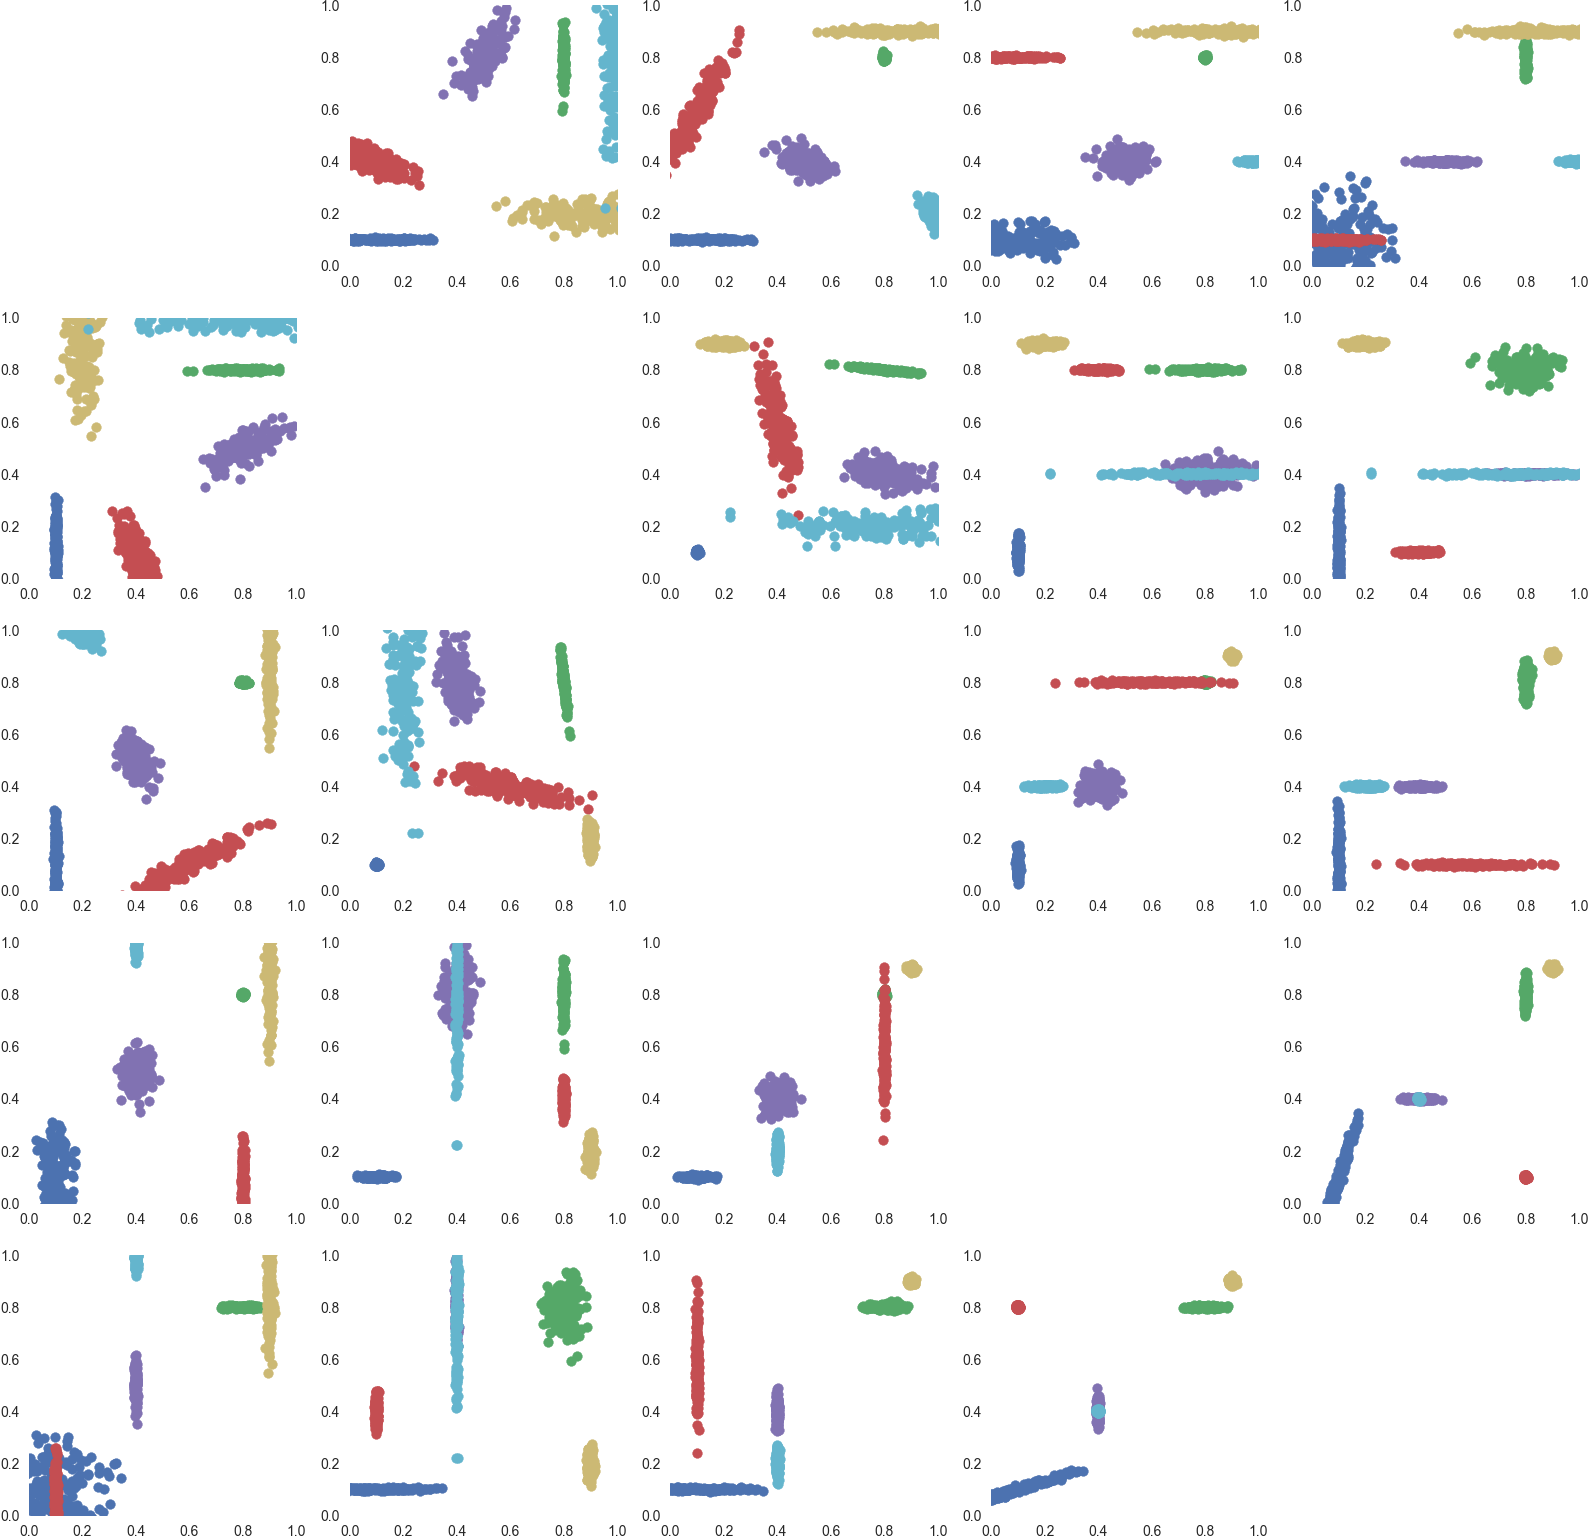
\includegraphics[width=\textwidth]{./TeX_files/experiments_data.png}
    \caption{Simulated data for the dictionary generator algorithm and KL-aggregation}
    \label{fig:experiments_data}
\end{figure}

\begin{figure}
\center
    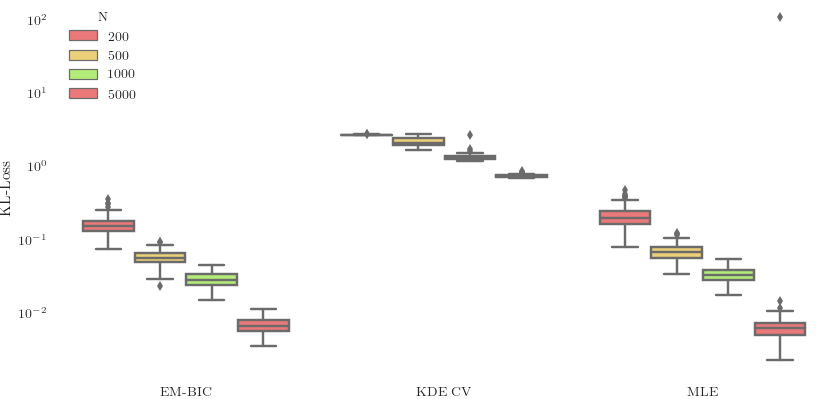
\includegraphics[width=0.8\textwidth]{./TeX_files/dict_gen_loss_dim_3_KL.png}
    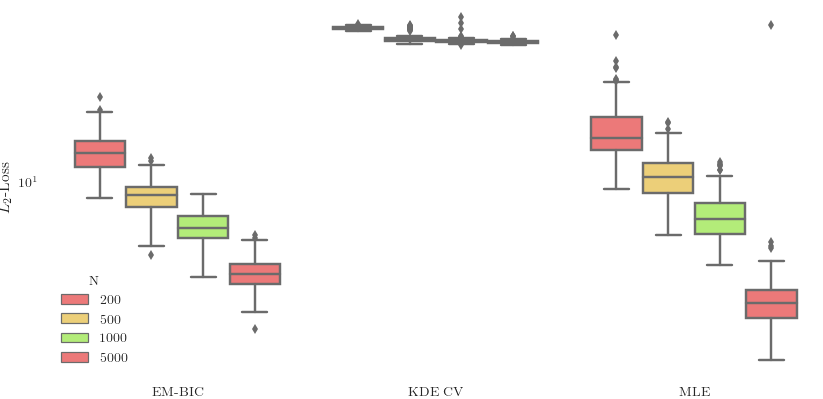
\includegraphics[width=0.8\textwidth]{./TeX_files/dict_gen_loss_dim_3_L2.png}
    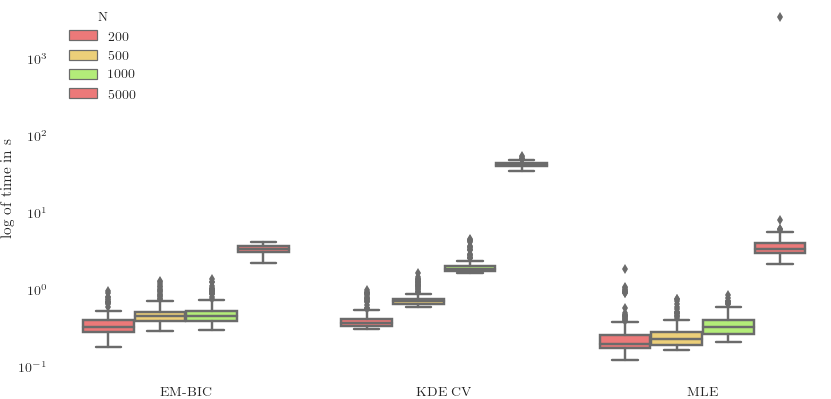
\includegraphics[width=0.8\textwidth]{./TeX_files/dict_gen_time_dim_3.png}
    \caption{Results for dimension 3. KL-Loss (upper panel), $L_2$-Loss (middle panel) and computation time (lower panel). Without dictionary generation optimizations.}
    \label{fig:result_dict_gen_dim_3}
\end{figure}
\begin{figure}
\center
    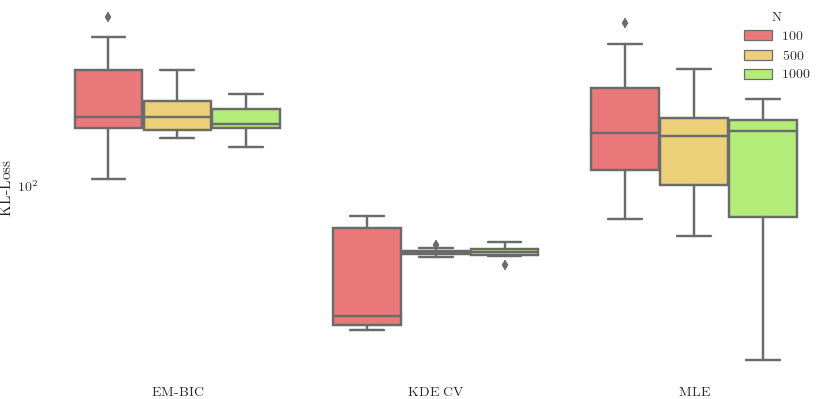
\includegraphics[width=0.8\textwidth]{./TeX_files/dict_gen_loss_dim_4_KL.png}
    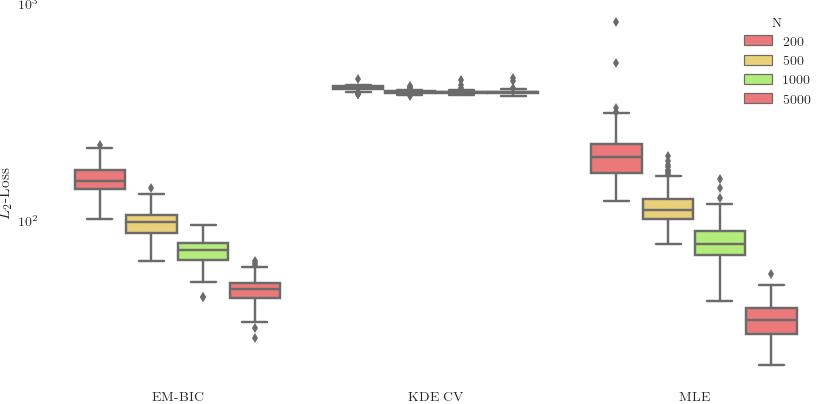
\includegraphics[width=0.8\textwidth]{./TeX_files/dict_gen_loss_dim_4_L2.png}
    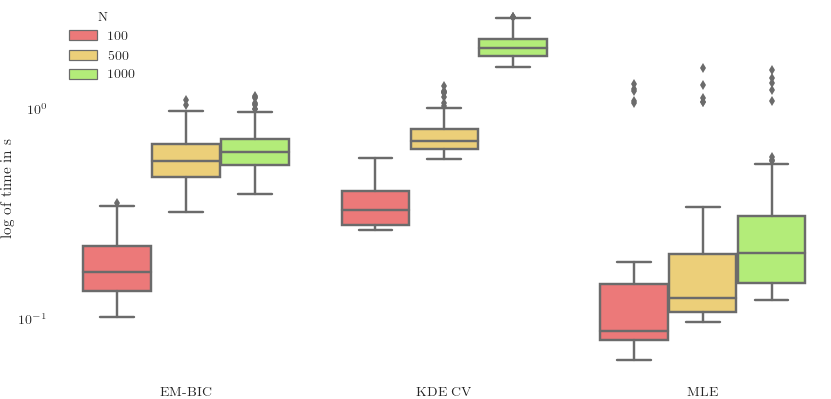
\includegraphics[width=0.8\textwidth]{./TeX_files/dict_gen_time_dim_4.png}
    \caption{Results for dimension 4. KL-Loss (upper panel), $L_2$-Loss (middle panel) and computation time (lower panel). Without dictionary generation optimizations.}
    \label{fig:result_dict_gen_dim_4}
\end{figure}
\begin{figure}
\center
    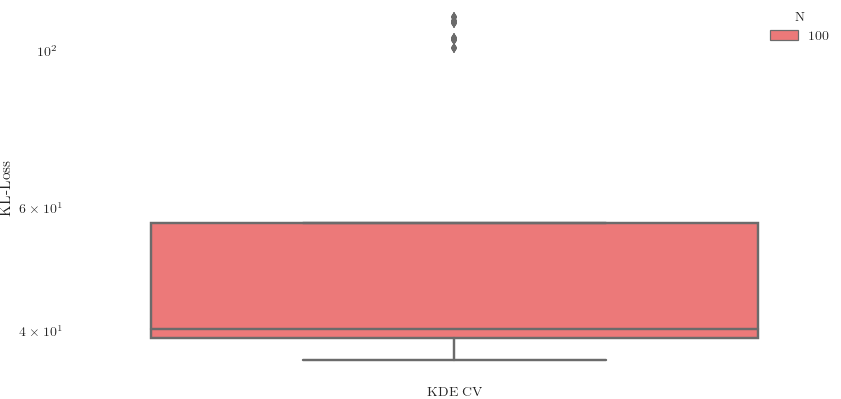
\includegraphics[width=0.8\textwidth]{./TeX_files/dict_gen_loss_dim_5_KL.png}
    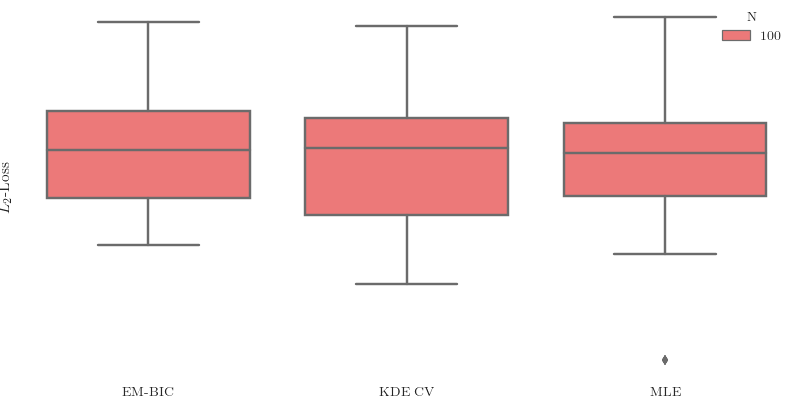
\includegraphics[width=0.8\textwidth]{./TeX_files/dict_gen_loss_dim_5_L2.png}
    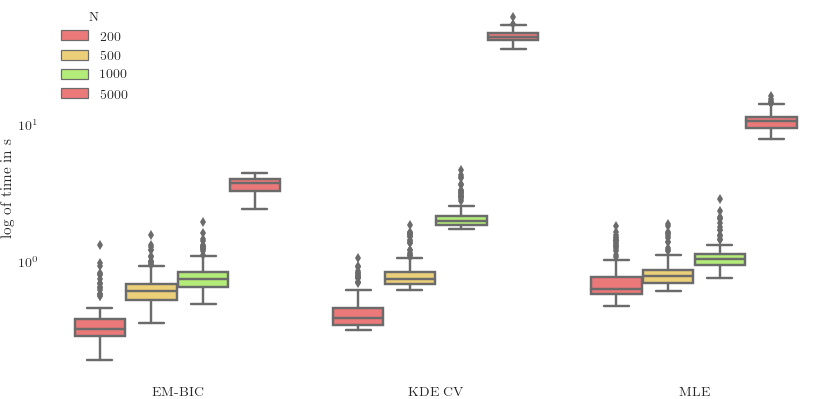
\includegraphics[width=0.8\textwidth]{./TeX_files/dict_gen_time_dim_5.png}
    \caption{Results for dimension 5. KL-Loss (upper panel), $L_2$-Loss (middle panel) and computation time (lower panel). Without dictionary generation optimizations.}
    \label{fig:result_dict_gen_dim_5}
\end{figure}
\subsubsection{Results with the selection of principal components and the goodness-of-fit test for the dictionary generator algorithm.}

Adding the two computation optimization techniques, our algorithm still performs better than KDE-CV and has similar performance than EM-BIC in $L_2$-loss (see  \Cref{fig:result_dict_gen_dim_3_gof_pc_select,fig:result_dict_gen_dim_4_gof_pc_select,fig:result_dict_gen_dim_5_gof_pc_select}). Unfortunately our method shows a bigger error variance for the KL-loss, especially when $N=5000$. This behavior is not expected and may be due to incorrect settings and subtleties in the implementation. Despite adding more  ``intelligence" in the construction of the dictionary, this procedures counterbalance the cost of adding too much densities to the KL-aggregation algorithm and therefore leads to smaller computational times independent of the size of the sample. Note that we implemented our methods in Python without Just-In-Time compilations and therefore suffers significant computation overhead compared to Numpy's implementation of EM-BIC and KDE-CV. We are confident that a proper optimized implementation would be significantly faster. This remark highlights the attractiveness of our methods when the size of the sample increases.
\begin{figure}
\center
    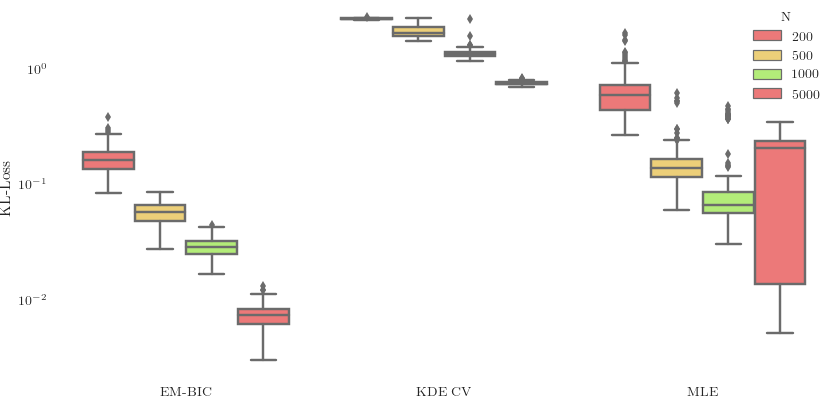
\includegraphics[width=0.8\textwidth]{./TeX_files/dict_gen_loss_dim_3_KL_gof_pc_select.png} 
    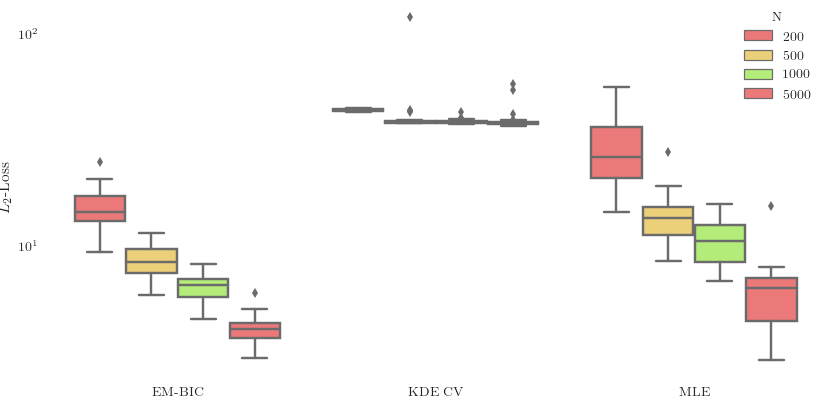
\includegraphics[width=0.8\textwidth]{./TeX_files/dict_gen_loss_dim_3_L2_gof_pc_select.png}
    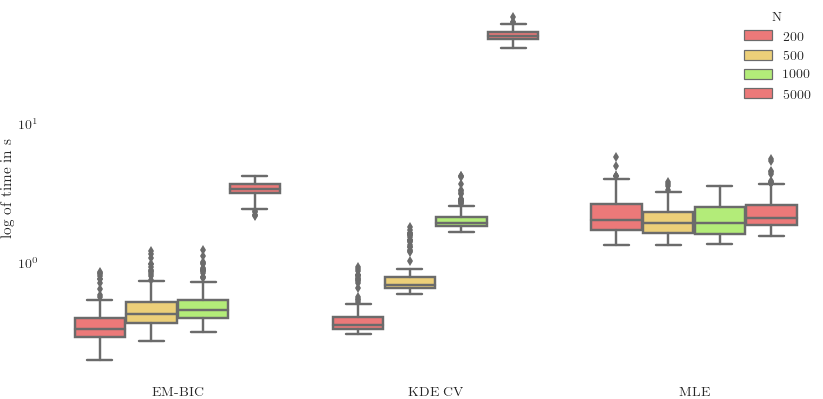
\includegraphics[width=0.8\textwidth]{./TeX_files/dict_gen_time_dim_3_gof_pc_select.png}
    \caption{Results for dimension 3. KL-Loss (upper panel), $L_2$-Loss (middle panel) and computation time (lower panel). With selection of principal components and deletion of similar densities.}
    \label{fig:result_dict_gen_dim_3_gof_pc_select}
\end{figure}
\begin{figure}
\center
    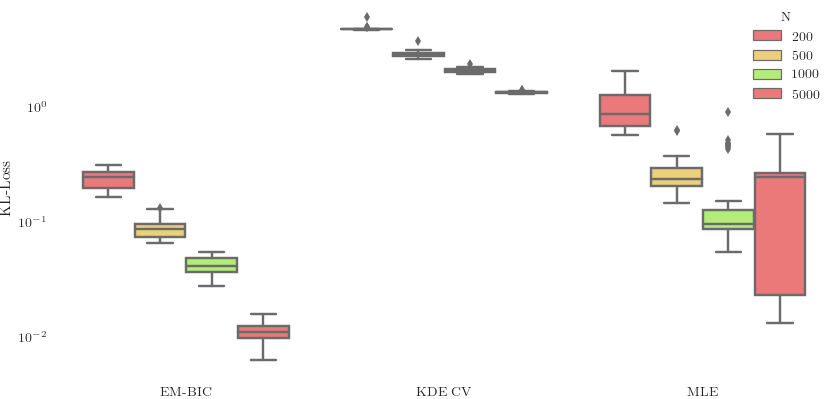
\includegraphics[width=0.8\textwidth]{./TeX_files/dict_gen_loss_dim_4_KL_gof_pc_select.png}
    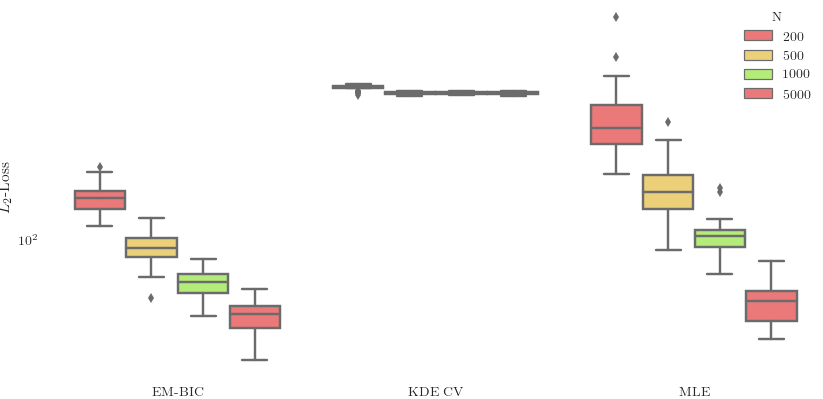
\includegraphics[width=0.8\textwidth]{./TeX_files/dict_gen_loss_dim_4_L2_gof_pc_select.png}
    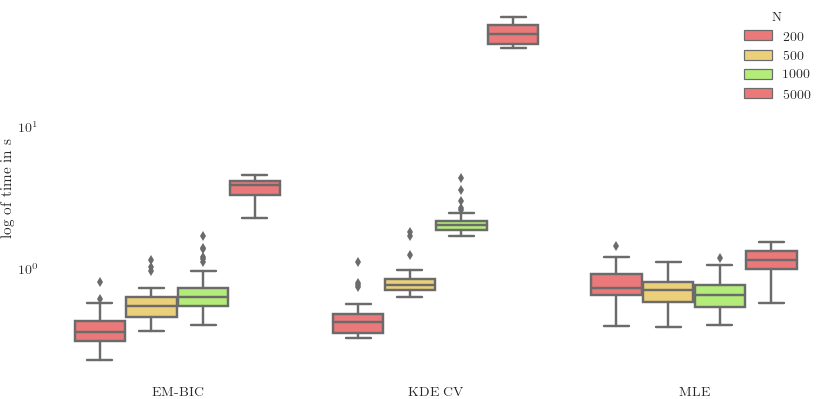
\includegraphics[width=0.8\textwidth]{./TeX_files/dict_gen_time_dim_4_gof_pc_select.png}
    \caption{Results for dimension 4. KL-Loss (upper panel), $L_2$-Loss (middle panel) and computation time (lower panel). With selection of principal components and deletion of similar densities.}
    \label{fig:result_dict_gen_dim_4_gof_pc_select}
\end{figure}
\begin{figure}
\center
    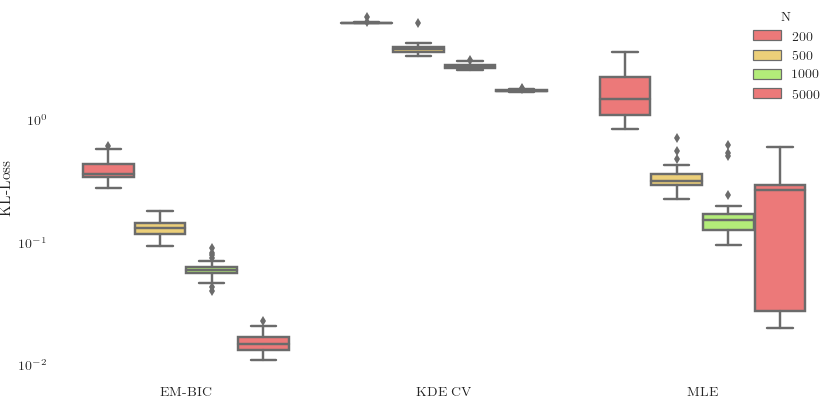
\includegraphics[width=0.8\textwidth]{./TeX_files/dict_gen_loss_dim_5_KL_gof_pc_select.png}
    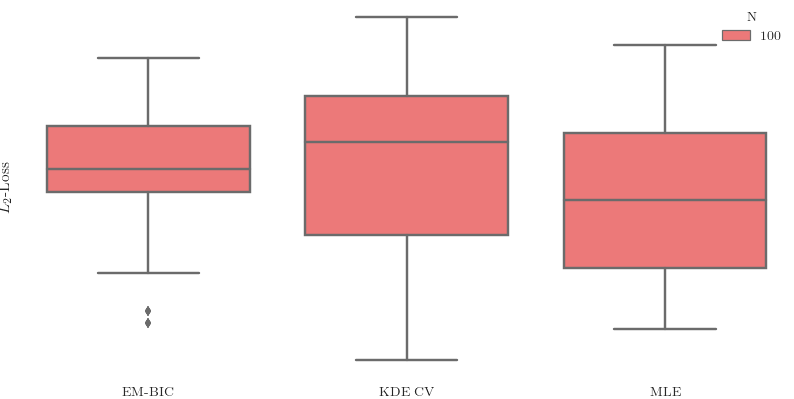
\includegraphics[width=0.8\textwidth]{./TeX_files/dict_gen_loss_dim_5_L2_gof_pc_select.png}
    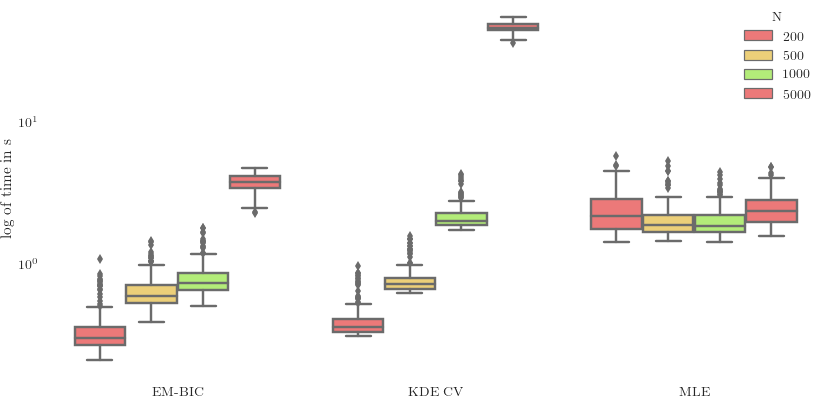
\includegraphics[width=0.8\textwidth]{./TeX_files/dict_gen_time_dim_5_gof_pc_select.png}
    \caption{Results for dimension 5. KL-Loss (upper panel), $L_2$-Loss (middle panel) and computation time (lower panel). With selection of principal components and deletion of similar densities.}
    \label{fig:result_dict_gen_dim_5_gof_pc_select}
\end{figure}
\subsection{Concluding remarks}
To conclude, the density dictionary generation method we developed is well suited for our KL-aggregation algorithm. Without the techniques that we implemented to lighten the density dictionary, our methods performs as well as EM-BIC in KL-loss and $L_2$-loss and slightly better with a large sample ($N=5000$). With the selection of principal components and the tests of similarity of densities in the dictionary, we tried to solve the problem of computational complexity of our method as the dimension and the size of the sample increase. On this setting, our method shows computation times independent of the size of the sample. Unfortunately, our algorithm shows a large error variance when $N=5000$ in KL-loss.  We are confident that a fine tuning of the parameters of the selection of principal components method and of the tests of similarity of densities would solve this problem.
Moreover, we observed in our simulations that the use of the selection of principal components technique and the tests of density similarities  to lighten the density dictionary gives us an estimation of the number of real clusters in the data and can be seen as a parameter-free clustering method. From this perspective, our method can be related to a subspace clustering method.